\documentclass[a4paper,12pt,twoside]{book}
\usepackage{lesi/lesi}


\title{Projeto de Desenvolvimento de Software}
\author{José Macedo, 12939 \AND Daniel Vilaça, 16939 \AND  Vitor Sá, 20484 \AND João Machado, 21151 \AND Jonatas de Paula, 22562}
\LESI
\regimePosLaboral
\date{\today}

\orientador{Nuno Rodrigues}

% comentar se não for para usar glossários
%\makeglossaries


% inicio do documento
\begin{document}
% 
\newglossaryentry{exemplo}
{
	name=exemplo,
	description={Exemplo de descrição}
}
 

\newacronym{ucpds}{PDS}{Projeto de Desenvolvimento de Software}

\newacronym{ucpw}{PW}{Programação Web}

\newacronym{uccd}{CD}{Comunicação de dados}

\newacronym{uc}{UC}{Unidade Curricular}

\newacronym{ucs}{UC's}{Unidadees Curriculares}

\newacronym{ipca}{IPCA}{Instituto Politécnico do Cávado e do Ave}



\frontmatter
\maketitle  % print the title

\begin{resumo}
Fazer um pequeno resumo sobre o projeto...
\end{resumo}

\tableofcontents

% comentar se nao tiver figuras
\listoffigures
\addcontentsline{toc}{chapter}{Lista de Figuras}

% Commentar proximas duas linhas se nao for para usar acronimos
\printglossary[type=\acronymtype,title={Siglas \& Acrónimos},toctitle={Siglas \& Acrónimos}]

% Commentar proximas duas linhas se nao for para usar glossarios
\printglossary[title={Indice de Termos},toctitle={Indice de Termos}]

% comentar se nao se quiser lista de listagens
%\lstlistoflistings
%\addcontentsline{toc}{chapter}{Lista de Código}

% comentar se não for para usar bibliografia
%\bibliography{biblio}
%\addcontentsline{toc}{chapter}{Bibliografia}

\mainmatter

% introdução

\chapter{Introdução}

A necessidade de automatizar e simplificar acompanham a necessidade de orzanizar os documentos e da sua rastreabilidade. A informatização dos processos administrativos são cada vez mais importantes nos dias de hoje de maneira a deixar mais tempo livre os intervenientes para outras tarefas que não sejam possiveis de informatizar. 

\section{Contexto}

Este projeto nasce no âmbito curricular, interligando as \acrshort{ucs} de \acrshort{ucpds} e \acrshort{ucpw}. Desta maneira nasce o projeto \textit{I-Library} que consiste em criar uma plataforma direcionada à biblioteca do IPCA de gestão e requisição de livros. 


\section{Objetivos}

O objetivo deste projeto é simular uma biblioteca online, onde é possivel fazer requisições de livros online, fazer pesquisa da database da biblioteca.

Facilitamos ao aluno um espaço online, onde não é preciso a presença do mesmo na biblioteca, e de manter um progresso e histórico dos livros que o mesmo requisitou, pesquisou ou até mesmo se esqueceu de entregar.

Facilitamos ao funcioário da biblioteca um espaço online, onde ele pode fazer um controlo do stock online e uniforme. Sendo online pode também dar baixa de livros e gerir com mais rapidez e eficácia todas as requisições ativas e coimas ativas da biblioteca.


Facilitamos ao admin/gestor da biblioteca um espaço online, onde tem todo o controlo sobre a biblioteca online, sem precisar de estar sempre presencialmente. Pode gerir os funcionários/alunos e todos os livros, requisições e coimas de toda a biblioteca com poucos cliques.



\clearpage

\section{Estrutura do documento}
Este documento agrupa toda a documentação produzida pelo grupo de trabalho em todas as fases do projeto.

\begin{enumerate}
	\item Produto. Contextualizar o problema e fazer o enquadramento do mesmo;

\end{enumerate}

\subsection*{\textbf{NOTA}:}

Cada um dos capítulos da lista anterior inclui ainda dados referentes a todas as reuniões do grupo de trabalho. A parte alfanumérica que identifica cada reunião corresponde a cada \textit{milestone} do projeto:
\begin{itemize}
	\item \textbf{ES} = Especificação;
	\item \textbf{MA} = Release Alpha;
	\item \textbf{MB} = Release Beta;
	\item \textbf{RTW} = Release to Web. . 
\end{itemize}

\newpage

\section{Equipa}

A composição do grupo de trabalho, nome do projeto, nome da equipa e cargos foi finalizada na primeira reunião (identificada como reunião MA01 transcrita no capítulo \ref{reuniaoMA01} na página \pageref{reuniaoMA01}).\\[4mm]

\noindent \textbf{Nome do projeto}\\
\noindent \rule{\linewidth}{0.4pt}
\noindent I-Library \\

\noindent \textbf{Nome da equipa}\\
\noindent \rule{\linewidth}{0.4pt}
\noindent 5Solutions \\

\noindent \textbf{Membros e cargos}\\
\noindent \rule{\linewidth}{0.4pt}
\noindent Vitor Sá (20484) \textbf{Product Owner}\\
\noindent Jonatas de Paula  (22562) \textbf{Scrum Master}\\
\noindent José Macedo (12939) Development team member\\
\noindent João Machado (21151) Development team member\\
\noindent Daniel Vilaça (16939) Development team member\\


% Release Especificação
\chapter{Especificação}

Neste capítulo abordaremos os aspetos referentes ao estudo de requisitos e regras de negócio concretizando-o com os diagramas de UML de modo a obter parametros necessários para o bom desenvolvimento do sistema.

\section{Casos de uso}

O diagrama de casos de uso permite documentar aquilo que o sistema é capaz de
efetuar a partir do ponto vista do utilizador final, sob forma de diagrama. Este tipo
de diagramas podem descrever as funções principais, funcionalidades do sistema e ainda
interações de funcionalidades com os seus utilizadores.
Deste modo, um diagrama de caso de uso, permite especficar o contexto, identficar
requisitos e validar a arquitetura de um dado sistema.

\newpage
%Casos de uso
\subsection{\labeltext[UC00 - Sistema]{UC-00 - Sistema}{uc:00}}
A imagem identificada como figura~\ref{fig:chap210} apresenta o diagrama de caso de uso \ref{uc:00} e tem como objetivo ilustrar de modo geral como o sistema funcionará.

\vspace*{5mm}

\begin{figure}[H]
	\centering
	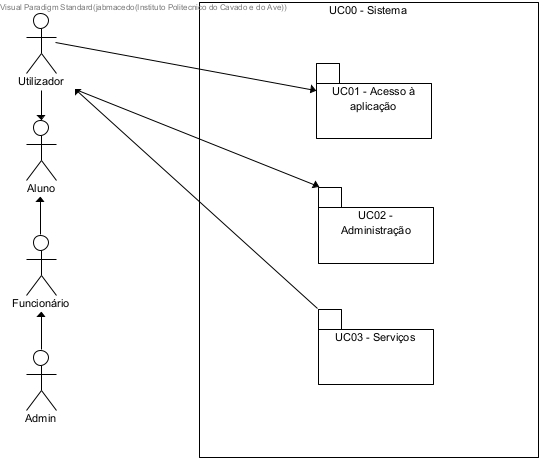
\includegraphics[width=1\linewidth]{./img/Diagramas\_UC/UC00.jpg}  % largura percentual 
	\caption{\ref{uc:00}}
	\label{fig:chap210}
\end{figure}

\par Tal como podemos observar na figura~\ref{fig:chap210}, consideramos que o nosso sistema está dividido em três grandes grupos de casos de uso, são:

\textbf{UC01 - Acesso a aplicação}  Aqui, iremos tratar os casos de uso referentes ao acesso à aplicação, tal como a criação de conta e autenticação do utilizador.

\textbf{UC02 - Administração}  Neste grupo, serão analisados os casos de uso referentes à gestão de conta e gestão de livros.

\textbf{UC03 - Serviços}  Para os serviços, tal como o nome indica iremos tratar abordar os casos de uso referente às requisições de livros, constultas e gestão de coimas.
\newpage

%UC01
\subsection{\labeltext[UC01 - Acesso ao sistema]{UC1.1 - Criar Conta}{uc:11}}
A imagem identificada como figura~\ref{fig:chap211} apresenta o diagrama de caso de uso \ref{uc:11} e tem como objetivo apresentar as interações entre os atores e o sistema.

\vspace*{5mm}

\begin{figure}[H]
	\centering
	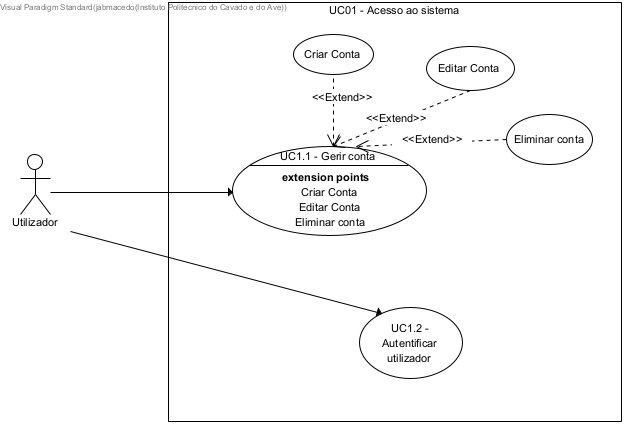
\includegraphics[width=1\linewidth]{./img/Diagramas\_UC/UC01.jpg}  % largura percentual 
	\caption{\ref{uc:11}}
	\label{fig:chap211}
\end{figure}

\noindent \textbf{Descrição} \\
\textbf{ID:} UC1.1 \\  
\textbf{Nível de importância:} Alta \\
\textbf{Nome:} Criar Conta \\
\textbf{Ator principal:} Utilizador \\
\textbf{Atores secundários:} --------- \\
\textbf{Breve descrição:} O utilizador para usar a aplicação deve criar conta. \\ 
\textbf{Ativador:} Iniciar a aplicação.  \\
\textbf{Pré-condições:} --------- \\
\textbf{Fluxo normal dos eventos:} \\
1. Abrir aplicação  \\
2. Clicar em registo de conta. \\
3. Preencher dados. \\
4. Carregar no botão "Registar"  \\
\textbf{Sub-fluxos:} --------- \\
\textbf{Fluxos alternativos/excecionais:}  \\
1. Erro de insersão de dados. \\

\subsection{UC1.2 - Autenticar utilizador}
\vspace*{5mm}

\noindent \textbf{Descrição} \\
\textbf{ID:} UC1.2 \\  
\textbf{Nível de importância:} Alta \\
\textbf{Nome:} Autenticar utilizador \\
\textbf{Ator principal:} Utilizador \\
\textbf{Atores secundários:} --------- \\
\textbf{Breve descrição:} O utilizador para usar o sistema deverá introduzir os dados de autenticação. A autenticação é validada com os dados da base de dados do sistema inseridos no ato da criação de conta. \\ 
\textbf{Ativador:} Utilizador autenticar-se.  Dados do utilizador registados na base de dados do sistema. \\
\textbf{Pré-condições:} Ter conta criada. \\
\textbf{Fluxo normal dos eventos:} \\
1. Abrir o sistema.  \\
2. Inserir email. \\
3. Inserir palavra-chave. \\
4. Carregar no botão "Login"  \\
\textbf{Sub-fluxos:} --------- \\
\textbf{Fluxos alternativos/excecionais:}  \\
1. Erro de autenticação, email ou palavra-chave incorretas. \\
\newpage

%UC02
\subsection{\labeltext[UC02 - Administração]{UC2.1 - Gerir Conta}{uc:21}}
A imagem identificada como figura~\ref{fig:chap212} apresenta o diagrama de caso de uso \ref{uc:21} e tem como objetivo apresentar as interações entre os atores e o sistema.

\vspace*{5mm}

\begin{figure}[H]
	\centering
	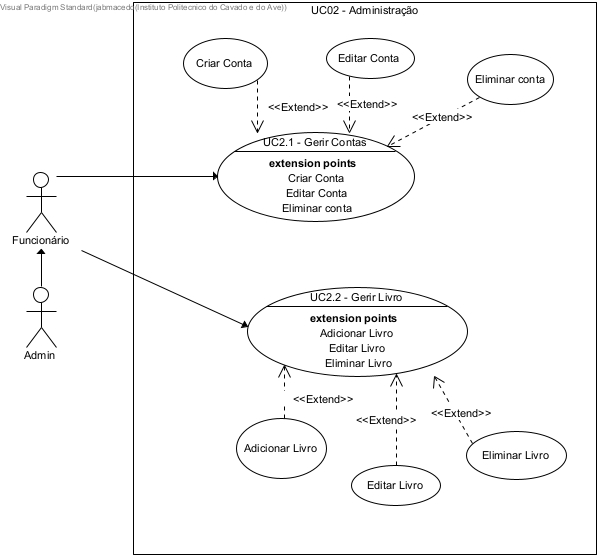
\includegraphics[width=1\linewidth]{./img/Diagramas\_UC/UC02.jpg}  % largura percentual 
	\caption{\ref{uc:21}}
	\label{fig:chap212}
\end{figure}

\newpage

\noindent \textbf{Descrição} \\
\textbf{ID:} UC2.1 \\  
\textbf{Nível de importância:} Alta \\
\textbf{Nome:} Gerir Conta \\
\textbf{Ator principal:} Utilizador \\
\textbf{Atores secundários:} --------- \\
\textbf{Breve descrição:} O utilizador poderá editar e eliminar conta. \\ 
\textbf{Ativador:} Intenção do utilizador querer editar a sua conta.  \\
\textbf{Pré-condições:} Ter conta criada. \\
\textbf{Fluxo normal dos eventos:} \\
1. Abrir sistema.  \\
2. Autenticar-se no sistema. \\
3. Selecionar "Conta" \\
\textbf{Sub-fluxos:} \\ 
\indent A - Editar conta\\
	\indent\indent A.1 - Este sub-fluxo inicia quando o utilizador deseja editar conta.\\
	\indent\indent A.2 - O utilizador insere os dados nos campos onde quer alterar.\\	
	\indent\indent A.3 - O utilizador carrega no botão "Registar".\\	
	\indent\indent A.4 - O sistema guarda os dados na base de dados e encaminha para o menu principal.\\	
	\indent B - Apagar conta \\ 
	\indent\indent B.1 - Este sub-fluxo inicia quando o utilizador deseja apagar a sua conta do sistema.\\
	\indent\indent B.2 - O sistema uma mensagem de confirmação da ação.\\
	\indent\indent B.3 - O utilizador confirma a operação.\\
	\indent\indent B.4 - O sistema guarda os dados na base de dados e encaminha o utilizador para a página inicial do sistema.\\
\textbf{Fluxos alternativos/excecionais:}  \\
	\indent A qualquer momento antes de submeter, o utilizador pode selecionar cancelar. A ação não é gravado e o caso de uso termina.\\
	\indent A - Editar conta\\
	\indent\indent A.5 - Se alguma informação estiver incorreta, o sistema pede ao utilizador para corrigir a informação.\\

\newpage

\subsection{UC2.2 - Gerir livro}
\vspace*{5mm}

\noindent \textbf{Descrição} \\
\textbf{ID:} UC2.2 \\  
\textbf{Nível de importância:} Alta \\
\textbf{Nome:} Gerir livro \\
\textbf{Ator principal:} Funcionário e/ou Administrador \\
\textbf{Atores secundários:} --------- \\
\textbf{Breve descrição:} O Funcionário e/ou Administrador deverão conseguir inserir, ediar e remover livros do sistema \\ 
\textbf{Ativador:} Necessidade do Funcionário e/ou Administrador dar entrada, editar dados e/ou apagar um livro. \\
\textbf{Pré-condições:} Ter nível de permissão de Funcionário e/ou Administrador. \\
\textbf{Fluxo normal dos eventos:} \\
	\indent Caso de uso inicia quando o Funcionário e/ou Administrador deseja gerir livros. \\
	\indent De acordo com o tipo de operação que deseja efetuar é encaminhado para os seguintes sub-fluxo:\\
	\indent\indent A - Se o utilizador deseja criar/inserir um livro, o sub-fluxo "Inserir" é executado.\\
	\indent\indent B - Se o utilizador deseja editar um livro, o sub-fluxo "Editar" é executado.\\
	\indent\indent C - Se o utilizador deseja remover um livro, o sub-fluxo "Remover" é executado.\\
\textbf{Sub-fluxos:} \\
	\indent A - Inserir livro\\
	\indent\indent A.1 - Este sub-fluxo inicia quando o utilizador deseja inserir um livro.\\
	\indent\indent A.2 - O utilizador insere os dados nos campos necessários.\\	
	\indent\indent A.3 - O utilizador carrega no botão "Registar".\\	
	\indent\indent A.4 - O sistema guarda os dados na base de dados e encaminha para o menu gerir livros.\\	
	\indent B - Editar livro \\ 
	\indent\indent B.1 - Este sub-fluxo inicia quando o utilizador deseja alterar informação de um livro.\\
	\indent\indent B.2 - É apresentado ao utilizador a lista de livros.\\
	\indent\indent B.3 - O utilizador edita os dados dos campos a editar.\\
	\indent\indent B.4 - O utilizador carrega no botão Atualizar.\\
	\indent\indent B.5 - O sistema guarda os dados na base de dados e encaminha para o menu gerir livros.\\
	\indent C -Remover livro  \\
	\indent\indent C.1 - Este sub-fluxo inicia quando o utilizador deseja remover um livro.\\
	\indent\indent C.2 - O sistema apresenta a lista de livros.\\
	\indent\indent C.3 - O utilizador seleciona livro que deseja remover.\\
	\indent\indent C.4 - O sistema responde com uma mensagem "livro removido com sucesso." e encaminha para o menu gerir livros.\\
\textbf{Fluxos alternativos/excecionais:}  \\
	\indent A qualquer momento antes de submeter, o utilizador pode selecionar cancelar. A ação não é gravado e o caso de uso termina.\\
	\indent A - Inserir livro\\
	\indent\indent A.5 - Se alguma informação estiver incorreta, o sistema pede ao utilizador para corrigir a informação.\\
	\indent B - Editar livro\\
	\indent\indent B.6 - Se alguma informação estiver incorreta, o sistema pede ao utilizador para corrigir a informação.\\
\newpage

%UC03
\subsection{\labeltext[UC03 - Serviços]{UC3.1 - Requisitar livro}{uc:31}}
A imagem identificada como figura~\ref{fig:chap213} apresenta o diagrama de caso de uso \ref{uc:31} e tem como objetivo apresentar as interações entre os atores e o sistema.

\vspace*{5mm}

\begin{figure}[H]
	\centering
	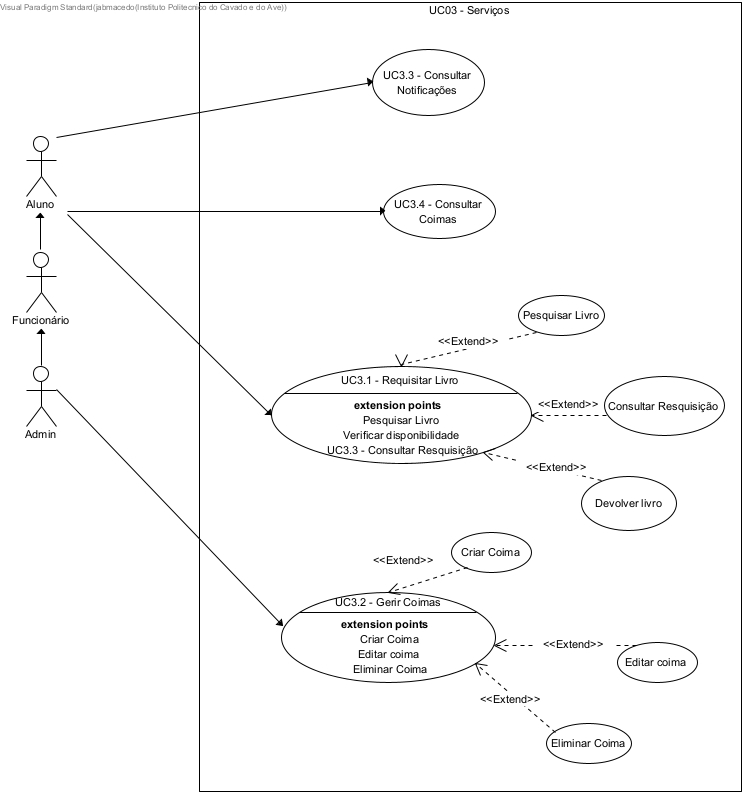
\includegraphics[width=1\linewidth]{./img/Diagramas\_UC/UC03.jpg}  % largura percentual 
	\caption{\ref{uc:31}}
	\label{fig:chap213}
\end{figure}

\newpage

\noindent \textbf{Descrição} \\
\textbf{ID:} UC3.1 \\  
\textbf{Nível de importância:} Alta \\
\textbf{Nome:} Requisitar livro \\
\textbf{Ator principal:} Aluno \\
\textbf{Atores secundários:} Funcionário, Administrador \\
\textbf{Breve descrição:} O aluno deverá conseguir requisitar livros. \\ 
\textbf{Ativador:} Intenção do aluno querer requisitar um livro.  \\
\textbf{Pré-condições:} Ter conta criada. \\
\textbf{Fluxo normal dos eventos:} \\
1. Abrir sistema.  \\
2. Autenticar-se no sistema. \\
3. Selecionar "Livros" \\
\textbf{Sub-fluxos:} \\ 
\indent A - Pesquisar livro\\
	\indent\indent A.1 - Este sub-fluxo inicia quando o utilizador deseja pesquisar um livro.\\
	\indent\indent A.2 - O sistema mostra a lista de livros.\\	
	\indent\indent A.3 - O utilizador insere o nome do livro a pesquisar.\\	
	\indent\indent A.4 - O utilizador carrega no botão "Pesquisar".\\	
	\indent\indent A.5 - O sistema mostra o resultado da pesquisa.\\	
	\indent\indent A.5 - O utilzador carrega no botão "Requisitar".\\
	\indent B - Devolver livro \\ 
	\indent\indent B.1 - Este sub-fluxo inicia quando o utilizador deseja devolver um livro.\\
	\indent\indent B.2 - O utilizador insere o livro a devolver e carrega "Devolver"\\
	\indent\indent B.3 - O sistema guarda os dados na base de dados e encaminha o utilizador para a página de requisição de livros.\\
	\indent C - Consultar requisção \\ 
	\indent\indent C.1 - Este sub-fluxo inicia quando o utilizador deseja consultar requisição de um livro.\\
	\indent\indent C.2 - O utilizador carrega no botão "Consultar resuisição".\\
	\indent\indent C.3 - O sistema devolve uma lista com as requisições do utilizador."\\
	\indent\indent C.4 - O utilizador carrega na requisição que deseja e é-lhe mostrada as informações sobre a requisição.\\
\textbf{Fluxos alternativos/excecionais:}  \\
	\indent A qualquer momento antes de submeter, o utilizador pode selecionar cancelar. A ação não é gravado e o caso de uso termina.\\

\newpage

\subsection{UC3.2 - Gerir coimas}
\vspace*{5mm}

\noindent \textbf{Descrição} \\
\textbf{ID:} UC3.2 \\  
\textbf{Nível de importância:} Alta \\
\textbf{Nome:} Gerir coimas \\
\textbf{Ator principal:} Administrador \\
\textbf{Atores secundários:} Funcionário \\
\textbf{Breve descrição:} O Administrador deverá conseguir criar, ediar e remover coimas do sistema. \\ 
\textbf{Ativador:} Necessidade do Administrador criar, editar ou remover uma coima.\\
\textbf{Pré-condições:} Ter nível de permissão de Administrador. \\
\textbf{Fluxo normal dos eventos:} \\
	\indent Caso de uso inicia quando o Administrador deseja gerir coimas. \\
	\indent De acordo com o tipo de operação que deseja efetuar é encaminhado para os seguintes sub-fluxo:\\
	\indent\indent A - Se o utilizador deseja criar/inserir coima, o sub-fluxo "Criar" é executado.\\
	\indent\indent B - Se o utilizador deseja editar uma coima, o sub-fluxo "Editar" é executado.\\
	\indent\indent C - Se o utilizador deseja remover uma coima, o sub-fluxo "Remover" é executado.\\
\textbf{Sub-fluxos:} \\
	\indent A - Criar coima\\
	\indent\indent A.1 - Este sub-fluxo inicia quando o utilizador deseja criar uma coima.\\
	\indent\indent A.2 - O utilizador insere os dados nos campos necessários.\\	
	\indent\indent A.3 - O utilizador com carrega no botão "Registar".\\	
	\indent\indent A.4 - O sistema guarda os dados na base de dados e encaminha para o menu gerir coimas.\\	
	\indent B - Editar coima \\ 
	\indent\indent B.1 - Este sub-fluxo inicia quando o utilizador deseja alterar informação de uma coima.\\
	\indent\indent B.2 - É apresentado ao utilizador a lista de coimas.\\
	\indent\indent B.3 - O utilizador edita os dados dos campos a editar.\\
	\indent\indent B.4 - O utilizador carrega no botão Atualizar.\\
	\indent\indent B.5 - O sistema guarda os dados na base de dados e encaminha para o menu gerir coimas.\\
	\indent C - Apagar coima  \\
	\indent\indent C.1 - Este sub-fluxo inicia quando o utilizador deseja apagar uma coima.\\
	\indent\indent C.2 - O sistema apresenta a lista de coimas.\\
	\indent\indent C.3 - O utilizador seleciona a coima que deseja apagar.\\
	\indent\indent C.4 - O sistema responde com uma mensagem "coima apagada com sucesso." e encaminha para o menu gerir coimas.\\
\textbf{Fluxos alternativos/excecionais:}  \\
	\indent A qualquer momento antes de submeter, o utilizador pode selecionar cancelar. A ação não é gravado e o caso de uso termina.\\
	\indent A - Criar coima\\
	\indent\indent A.5 - Se alguma informação estiver incorreta, o sistema pede ao utilizador para corrigir a informação.\\
	\indent B - Editar coima\\
	\indent\indent B.6 - Se alguma informação estiver incorreta, o sistema pede ao utilizador para corrigir a informação.\\

\newpage

\newpage

\subsection{UC3.3 - Consultar notificações}
\vspace*{5mm}

\noindent \textbf{Descrição} \\
\textbf{ID:} UC3.2 \\  
\textbf{Nível de importância:} Média \\
\textbf{Nome:} Consultar notificações \\
\textbf{Ator principal:} Aluno \\
\textbf{Atores secundários:} --------- \\
\textbf{Breve descrição:} O aluno deverá conseguir consultar as notificações que lhe são enderessadas. \\ 
\textbf{Ativador:} Necessidade do aluno querer consultar as notificações.\\
\textbf{Pré-condições:} Autenticar-se no sistema. \\
\textbf{Fluxo normal dos eventos:} \\
	\indent Caso de uso inicia quando o aluno deseja consultar as notificações. \\
	\indent O aluno clica em "Notificações".
	\indent O sistema devolve as notificações correspondentes.
\textbf{Sub-fluxos:} ---------\\
\textbf{Fluxos alternativos/excecionais:}  \\
	\indent A qualquer momento antes de submeter, o aluno pode selecionar cancelar. A ação não é gravado e o caso de uso termina.\\

	\subsection{UC3.4 - Consultar coimas}
\vspace*{5mm}

\noindent \textbf{Descrição} \\
\textbf{ID:} UC3.2 \\  
\textbf{Nível de importância:} Média \\
\textbf{Nome:} Consultar coimas \\
\textbf{Ator principal:} Aluno \\
\textbf{Atores secundários:} --------- \\
\textbf{Breve descrição:} O aluno deverá conseguir consultar as coimas que lhe são enderessadas. \\ 
\textbf{Ativador:} Necessidade do aluno querer consultar as coimas.\\
\textbf{Pré-condições:} Autenticar-se no sistema. \\
\textbf{Fluxo normal dos eventos:} \\
	\indent Caso de uso inicia quando o aluno deseja consultar as coimas. \\
	\indent O aluno clica em "Coimas".
	\indent O sistema devolve as coimas correspondentes.
\textbf{Sub-fluxos:} ---------\\
\textbf{Fluxos alternativos/excecionais:}  \\
	\indent A qualquer momento antes de submeter, o aluno pode selecionar cancelar. A ação não é gravado e o caso de uso termina.\\

\newpage
\newpage

%Modelo ER
\section{\labeltext[Diagrama de Entidade-Relação]{Diagrama de Entidade-Relação}{er:22}}

De forma a garantir um bom funcionamento e estabilidade para o sistema, é necessário desenvolver uma base de dados com capacidade de gestão e armazenamento de todos os dados, não apenas necessários para as requisições definidas inicialmente como também para uma possivel futura adição.
Para garantir isso realizamos o seguinte diagrama de entidade - relações, ou ER.

\begin{figure}[H]
	\centering
	\includegraphics[width=1\linewidth]{./img/Diagrama\_ER/Diagrama\_ER.png}  % largura percentual 
	\caption{\ref{er:22}}
	\label{fig:chap220}
\end{figure}

Neste sistema, e com as atuais requisições as tabelas principais deste diagrama são as tabelas, "User", "Requisição", "Multa" e "Livro", que interligam-se e complementam-se com outras tabelas mais pequenas ou intermediárias na comunicação entre duas das principais.

\par Como podemos observar na imagem, relativamente ao Utilizador, o mesmo possui uma serie de Atributos como o nome, email, password... e 2 chaves estrangeiras que apontam para 2 outras tabelas, "Curso" e "User\_Tipo" que armazenam todos os cursos e todos os possiveis tipos de user.
Observamos então que a tabela "User" se encontra diretamente conectada com a tabela "Requisição" sendo o "codUser" (chave primária da tabela User) uma chave estrangeira nessa tabela para garantir que a requisição se mantem relacionada com apenas um utilizador de forma mais automatizada e consistente.

\par A tabela "Requisição", também se relaciona com a tabela "Multa", é da tabela "Requisição" que será verificada a necessidade de aplicação de uma multa e calculado o custo da mesma com base nos dias em atraso, estes dados sao armazenados na tabela "Multa" interligada com  a tabela Requisição pela chave estrangeira "codRequisicao".

\par Para ser feito o pagamento da multa, ligamos a tabela "Multa" à tabela "Pagamento" que por sua vez se liga à tabela "Multibanco" e "MbWay", isto foi feito para que para cada multa fosse guardado apenas um Pagamento e os dados relativos ao mesmo, desta forma evita-se melhor o registo de 2 pagamentos por Multa e também podemos verificar estatisticamente o metodo mais utilizado de forma mais simples, com uma comparação entre as tabelas "MbWay" e "Multibanco" e observando qual tem o maior numero de registos.

\par Relativamente à tabela "Livro", a mesma está ligada à tabela "Exemplar", a tabela "Livro" armazena todos os dados de um titulo, a tabela "Exemplar", por sua vez, armazena todos os dados adicionais de um determinado volume.
Ambas as tabelas acima referidas estão ligadas a duas tabelas mais simples e pequenas respetivamente. A tabela "Livro" está ligada à tabela "Livro\_Tipo" de onde herda uma chave estrageira que aponta para o tipo de livro que é (ex: Romance, Ação, Ficção). A tabela "Exemplar, por sua vez, está ligada à tabela "Estado" de onde herda a chave estrangeira "codEstado" que aponta para o estado do exemplar (perdido, novo, como novo, com marcas de uso...).

\par Todas estas tabelas possuem uma parte importante para garantir um bom funiconamento de todas as requisições e como tal nenhuma das mesmas pode ser deixada de parte.

\newpage

%Diagramas de Classes
\subsection*{Mockups}


\newpage

%Diagramas de Atividades
\section{Diagrama de Entidade Relações}

De forma a garantir um bom funcionamento e estabilidade para o sistema, é necessário desenvolver uma base de dados com capacidade de gestão e armazenamento de todos os dados, não apenas necessários para as requisições definidas inicialmente como também para uma possivel futura adição.
Para garantir isso realizamos o seguinte diagrama de entidade - relações, ou ER.

imagem

Neste sistema, e com as atuais requisições as tabelas principais deste diagrama são as tabelas, "User", "Requisição", "Multa" e "Livro", que interligam-se e complementam-se com outras tabelas mais pequenas ou intermediárias na comunicação entre duas das principais.

Como podemos observar na imagem, relativamente ao Utilizador, o mesmo possui uma serie de Atributos como o nome, email, password... e 2 chaves estrangeiras que apontam para 2 outras tabelas, "Curso" e "User_Tipo" que armazenam todos os cursos e todos os possiveis tipos de user.
Observamos então que a tabela "User" se encontra diretamente conectada com a tabela "Requisição" sendo o "codUser" (chave primária da tabela User) uma chave estrangeira nessa tabela para garantir que a requisição se mantem relacionada com apenas um utilizador de forma mais automatizada e consistente.
A tabela "Requisição", também se relaciona com a tabela "Multa", é da tabela "Requisição" que será verificada a necessidade de aplicação de uma multa e calculado o custo da mesma com base nos dias em atraso, estes dados sao armazenados na tabela "Multa" interligada com  a tabela Requisição pela chave estrangeira "codRequisicao".
Para ser feito o pagamento da multa, ligamos a tabela "Multa" à tabela "Pagamento" que por sua vez se liga à tabela "Multibanco" e "MbWay", isto foi feito para que para cada multa fosse guardado apenas um Pagamento e os dados relativos ao mesmo, desta forma evita-se melhor o registo de 2 pagamentos por Multa e também podemos verificar estatisticamente o metodo mais utilizado de forma mais simples, com uma comparação entre as tabelas "MbWay" e "Multibanco" e observando qual tem o maior numero de registos.

Relativamente à tabela "Livro", a mesma está ligada à tabela "Exemplar", a tabela "Livro" armazena todos os dados de um titulo, a tabela "Exemplar", por sua vez, armazena todos os dados adicionais de um determinado volume.
Ambas as tabelas acima referidas estão ligadas a duas tabelas mais simples e pequenas respetivamente. A tabela "Livro" está ligada à tabela "Livro_Tipo" de onde herda uma chave estrageira que aponta para o tipo de livro que é (ex: Romance, Ação, Ficção). A tabela "Exemplar, por sua vez, está ligada à tabela "Estado" de onde herda a chave estrangeira "codEstado" que aponta para o estado do exemplar (perdido, novo, como novo, com marcas de uso...).

Todas estas tabelas possuem uma parte importante para garantir um bom funiconamento de todas as requisições e como tal nenhuma das mesmas pode ser deixada de parte.
\newpage

%Diagramas de Estados
\section{Diagrama de Estados}

\par O diagrama de estado representa os possíveis estados, sendo alterado pelas operações que são executados dentro do sistema I-Library.

\subsection{\labeltext[Diagrama de Estados - Levantamento]{Diagrama de estados - Levantamento}{es:250}}

\begin{figure}[H]
	\centering
	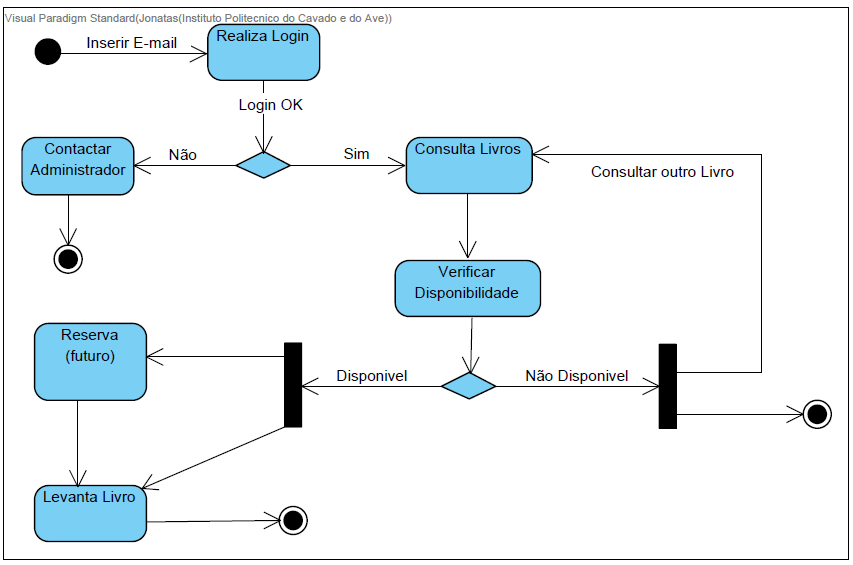
\includegraphics[width=1\linewidth]{./img/Diagrama_E/DE_Requisicao.png}  % largura percentual 
	\caption{\ref{es:250}}
	\label{fig:chap250}
\end{figure}

\par O diagrama de “Levantamento” inicia no estado "Realiza login", na falha de login o estado altera para “Contactar Administrador” e, após o processo finaliza, no caso de os dados estarem corretos o estado altera para “Consulta Livros”, após a ação do usuário o estado altera para “Verificar Disponibilidade”, deste momento, temos dois estados distintos, ou seja, caso tenha disponibilidade o estado altera para “Reserva Futuras” e após para “Levanta Livro”, neste sentido o estado finaliza, no caso de não haver disponibilidade o estado para altera para o fim.

%DE_Devolução
\subsection{\labeltext[Diagrama de Estados - Devolução]{Diagrama de estados - Devolução}{es:251}}

\begin{figure}[H]
	\centering
	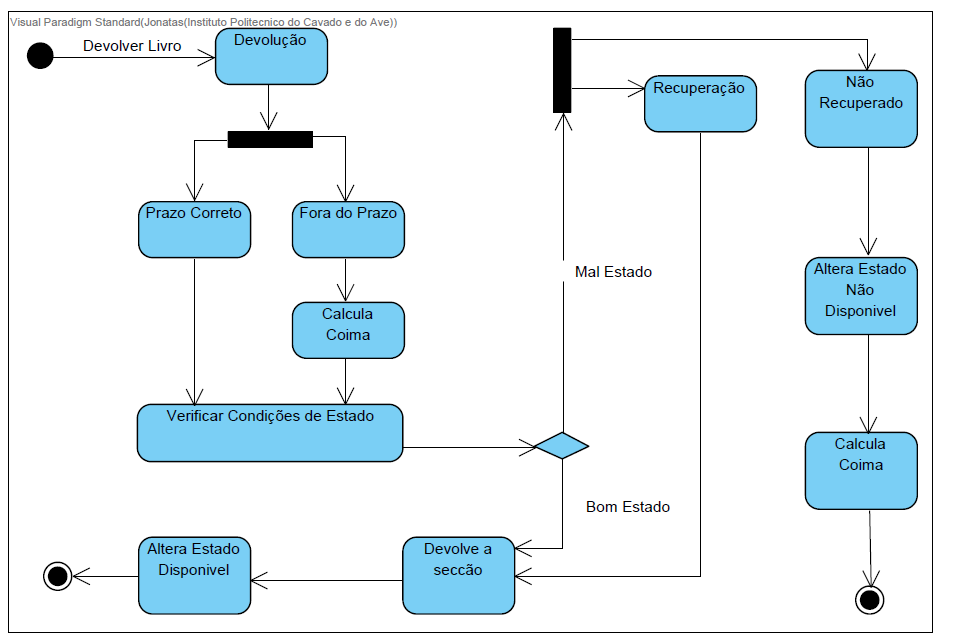
\includegraphics[width=1\linewidth]{./img/Diagrama_E/DE_Devolucao.png}  % largura percentual 
	\caption{\ref{es:251}}
	\label{fig:chap251}
\end{figure}

\par O diagrama de “Devolução” inicia no estado "Devolução", quando este está no “Prazo Correto” o estado segue para “Verificar condições de Estado”, na ocasião de estar “Fora do Prazo” o estado altera para “Calcula Coima”  e, segue para “Verificar condições de Estado”, quando este livro está em boas condições o estado altera para “Devolve a Secção” e após “Altera Estado para Disponível” e finaliza o processo, quando o livro encontra-se em mal condição o estado altera para “Recuperação” e caso seja possível o reparo volta para o estado de “Devolve a Secção”, já no caso de “Não Recuperado” o estado “Altera Estado para Não Disponível” e segue para “Calcula Coima” após o processo finaliza.

\newpage

%DE_Pagamento
\subsection{\labeltext[Diagrama de Estados - Pagamento]{Diagrama de estados - Pagamento}{es:252}}

\begin{figure}[H]
	\centering
	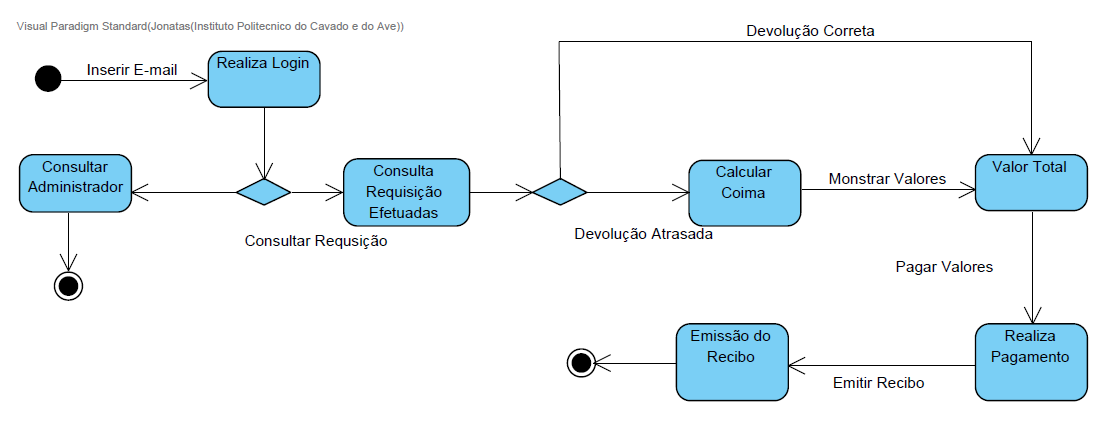
\includegraphics[width=1\linewidth]{./img/Diagrama_E/DE_Pagamento.png}  % largura percentual 
	\caption{\ref{es:252}}
	\label{fig:chap252}
\end{figure}

\par O diagrama de “Pagamento” inicia no estado de "Realiza login", na falha de login o estado altera para “Contactar Administrador” e, após o processo finaliza, no caso de login correto o estado altera “Consulta Requisição Efetuadas” neste momento o usuário terá acesso a todas suas requisições e, no caso de devolução atrasada o estado altera para “Calcular Coima” onde altera o estado para “Valor Total”, deste modo, o sistema altera o estado para “Realiza Pagamento”, após efetuado altera para “Emissão do Recibo”, sendo após finalizado o processo.

\newpage
\newpage

%Diagrama de Sequência
\section{Diagrama de Atividades}

Através dos diagramas de atividades a seguir representados, podemos ilustrar e entender melhor o fluxo de trabalho entre o user e o sistema, assim como melhor entender a lógica do funcionamento do mesmo.

imagem atividade user

Pelo diagrama acima apresentado, podemos ver que o utilizador pode utilizar o sistema com ou sem login, porém apenas com o login executado é possivel ao mesmo usufruir de todas as vantágens do web-service. O mesmo é aplicado a todos os outros users, apenas com o login é possivel desbloquear todas as funcionalidades disponiveis.
No caso do utilizador podemos ver que as opções são maioritáriamente de consulta, permitindo ao mesmo fazer uma gestão pessoal dos livros requisitados, coimas e ver todos os livros disponiveis.
O utilizador, enquanto aluno, pode, dentro de todos estes campos, realizar ações mais aprofundadas como a realizar a requisição de um determinado livro, e anular ou alterar a data da mesma até 24horas antes da data de levantamento e fazer o pagamento de multas.
A devolução do exemplar é feita de forma fisica, e é registada pelo funcionario ou admin.

imagem atividade funcionario

Com base no diagrama de atividade do funcionário, presente acima, é possivel observar que o mesmo possui um esquema identico ao do utilizador com apenas algumas adições e ligeiras alterações.
Um bom exemplo de uma alteração é quando observamos a consulta de requisições, já não sendo necessário o prazo de até 24h.
Quanto a funcionalidades adicionais, as principais são relativas aos exemplares/livros, o funcionario pode alertar o admin quanto ao estado de um determinado exemplar para que o admin possa proceder quanto ao tratamento dessa informação da melhor forma, e pode também alterar certos dados do livro, como o titulo, descrição, entre outros.

imagem admin

Como era de esperar, o administrador da biblioteca, ou qualquer user com o tipo admin, ter acesso ao maior numero de funcionalidades e maior liberdade de manipulação de dados.
O Admin pode realizar a eliminação de exemplares e livros, alterações manuais aos seus estados, assim como anular coimas, anular/alterar requisições, entre outras.
A maioria das funcionalidades são identicas para todos os utilizadores como o registo de uma requisição, a forma como as mesmas são geridas, consulta dos livros, consulta das coimas e a gestão das mesmas, sendo apenas aplicadas determinadas regras de negócio que permitem a existencia de uma hierarquia de ações que podem, se mal geridas, corromper todo o sistema.

\newpage

%Mockups
\section{Mockups}



\subsection{\labeltext[Ecrã - Home]{Ecrã - Home}{mo:270}}

Esta será a primeira pagina do nosso frontend. A home página com as funcionalidades do nosso projeto, na parte de cima um "Header" que é comum a todas as páginas da aplicação e na parte de baixo um "Footer" que também aparece em todas as páginas, com um logo do IPCA.

\begin{figure}[H]
	\centering
	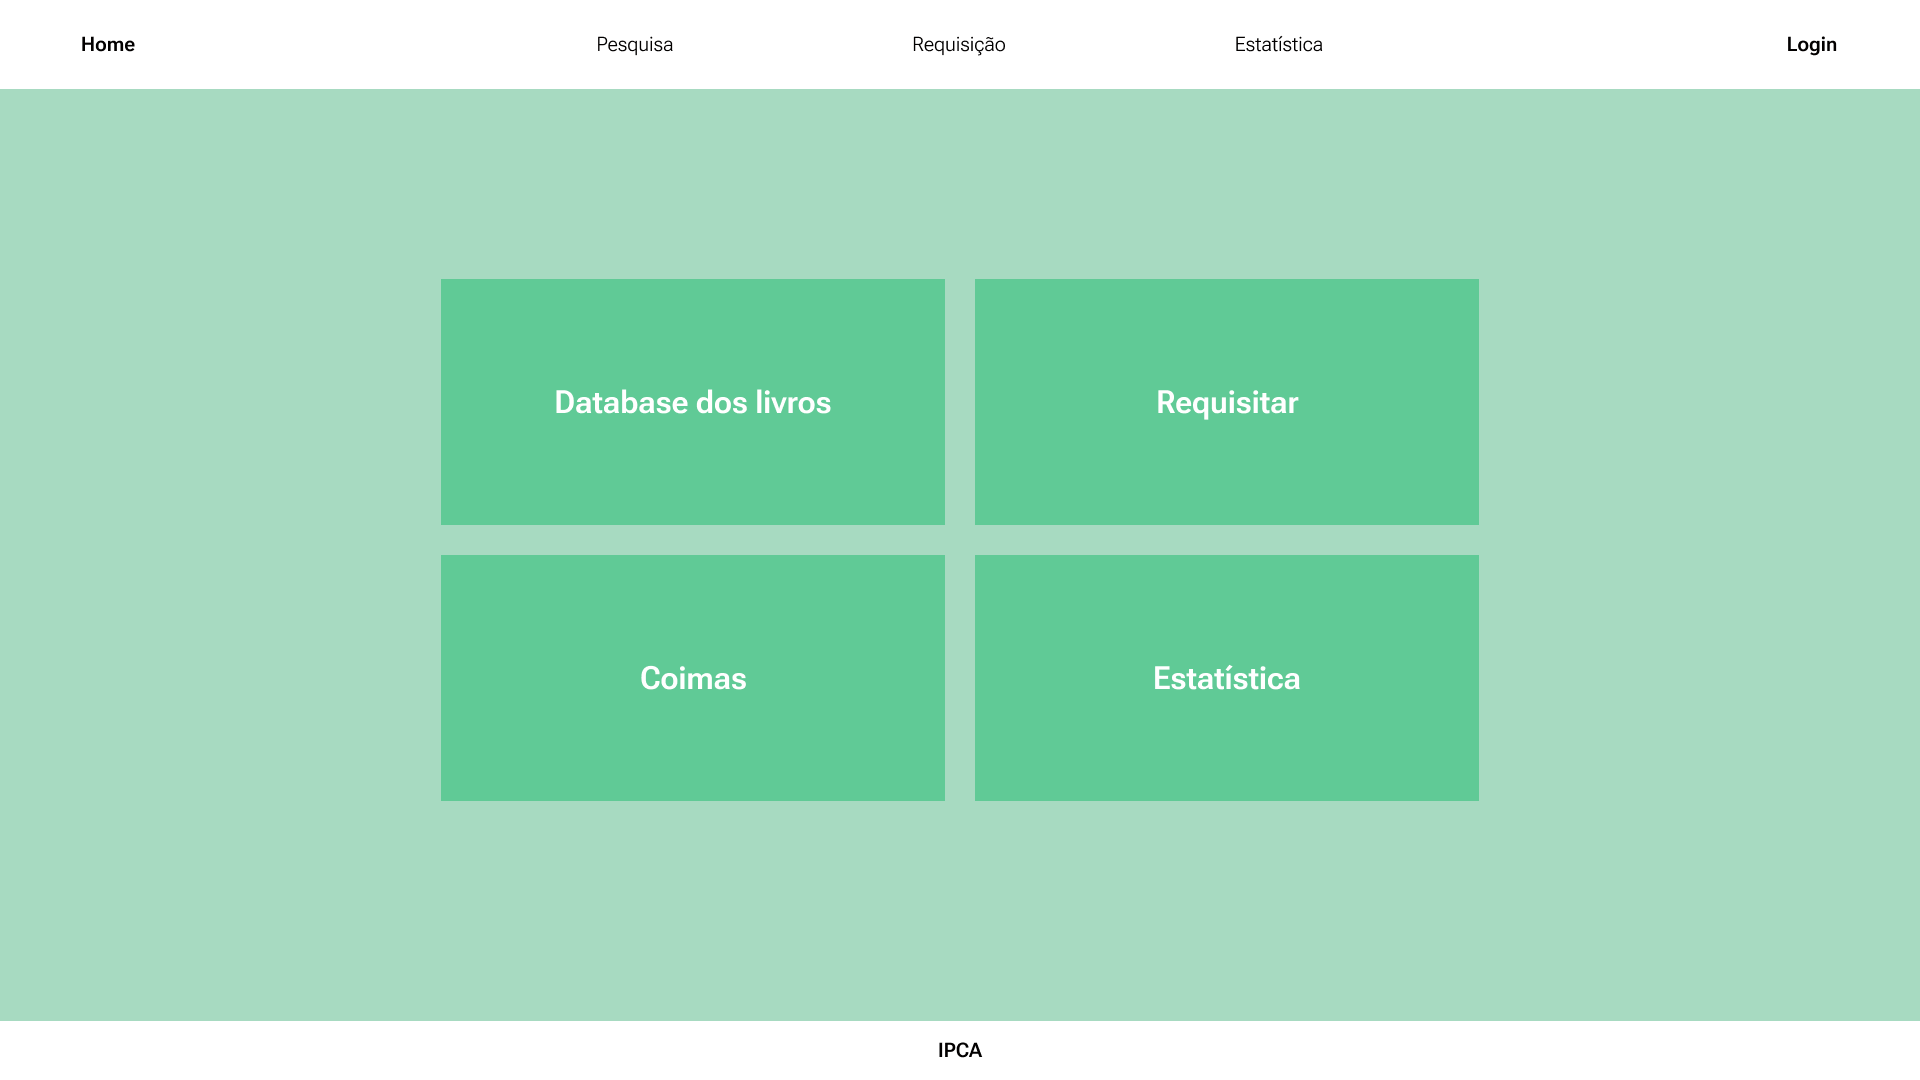
\includegraphics[width=1\linewidth]{../Mockups/PNGs/Home.png}  % largura percentual 
	\caption{\ref{mo:270}}
	\label{fig:chap270}
\end{figure}


\newpage 

\subsection{\labeltext[Ecrã - Sign Up]{Ecrã - Sign Up}{mo:271}}

Nesta página será onde o utilizador faz o seu registo/login. O aluno/funcionario/admin introduzem os seus dados de acesso, e no caso de se esquecerem da password, clicam no texto correspondente.

\begin{figure}[H]
	\centering
	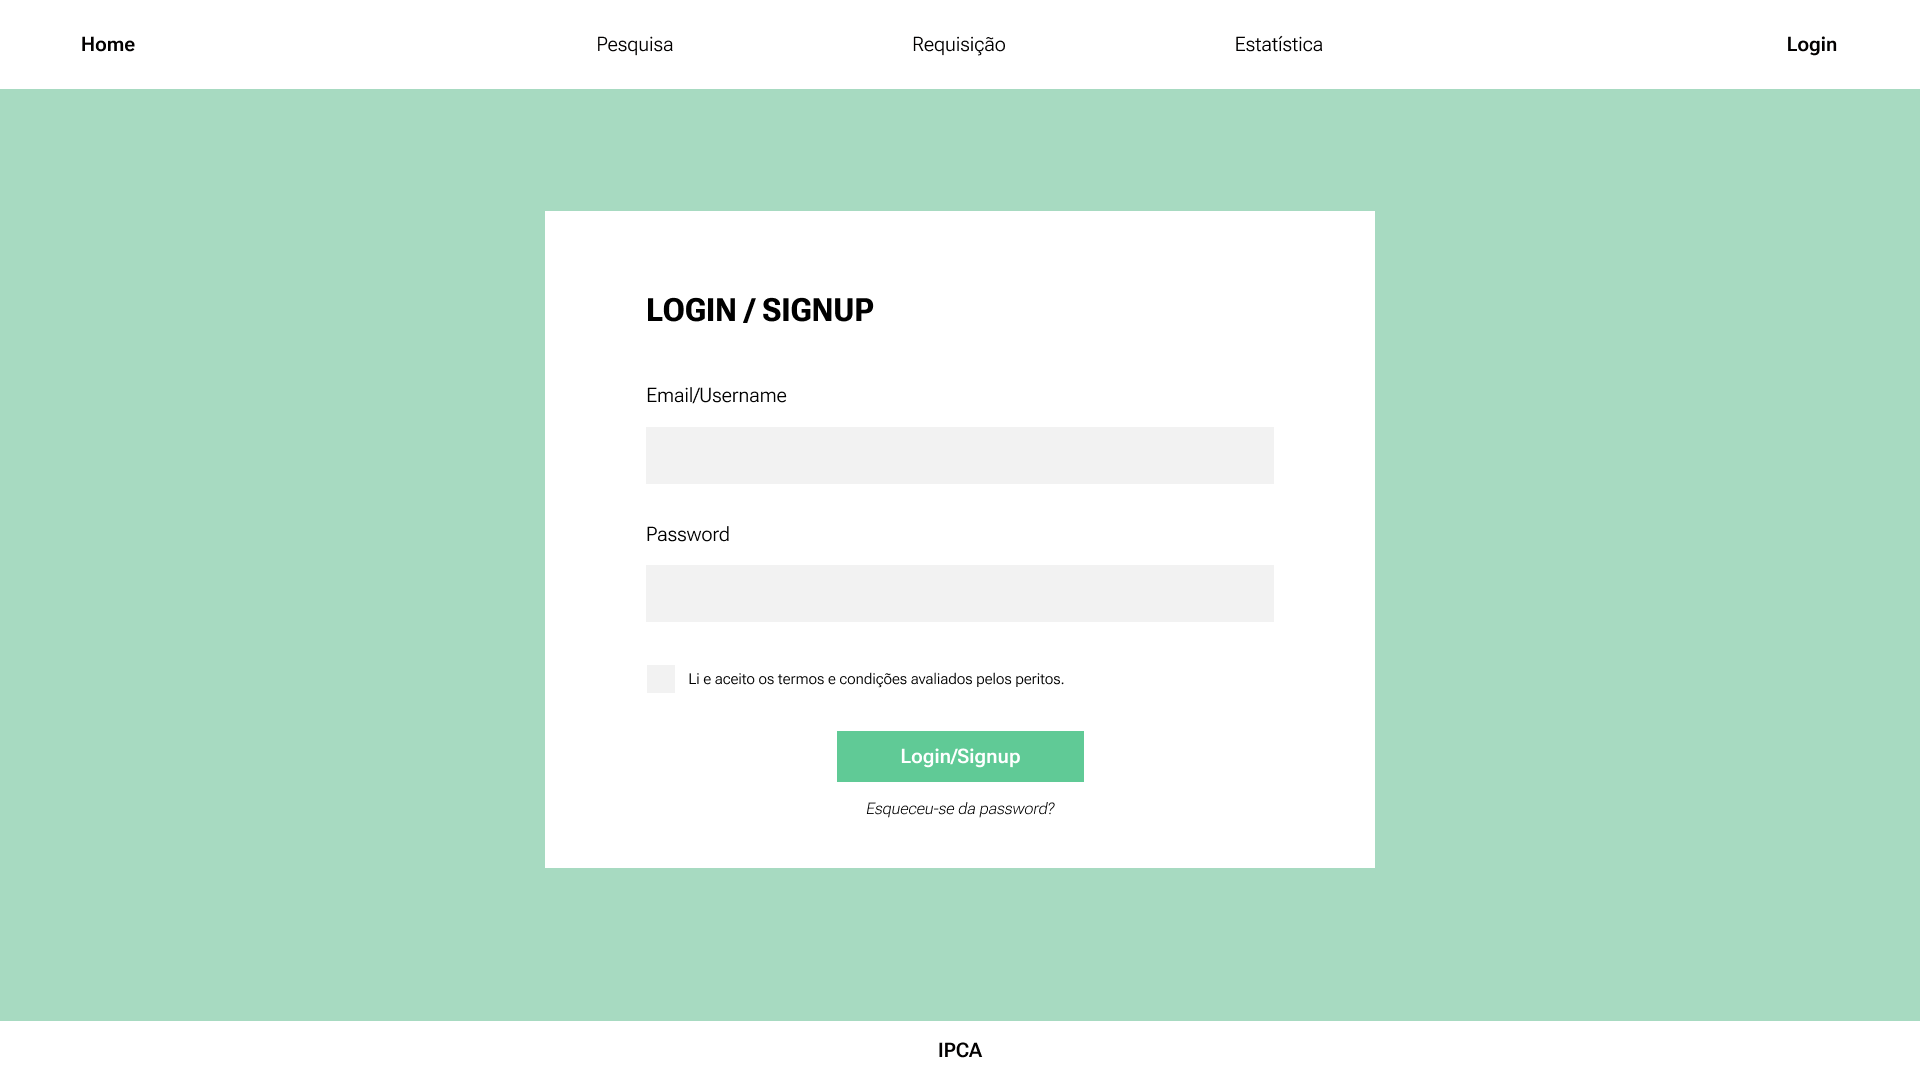
\includegraphics[width=1\linewidth]{../Mockups/PNGs/Login - Signup.png}  % largura percentual 
	\caption{\ref{mo:271}}
	\label{fig:chap271}
\end{figure}


\newpage 

\subsection{\labeltext[Ecrã - Login]{Ecrã - Login}{mo:272}}

Página onde os alunos/funcionarios/admin se encontram, se esquecerem da sua password. Necessita sempre do email por termos de segurança.

\begin{figure}[H]
	\centering
	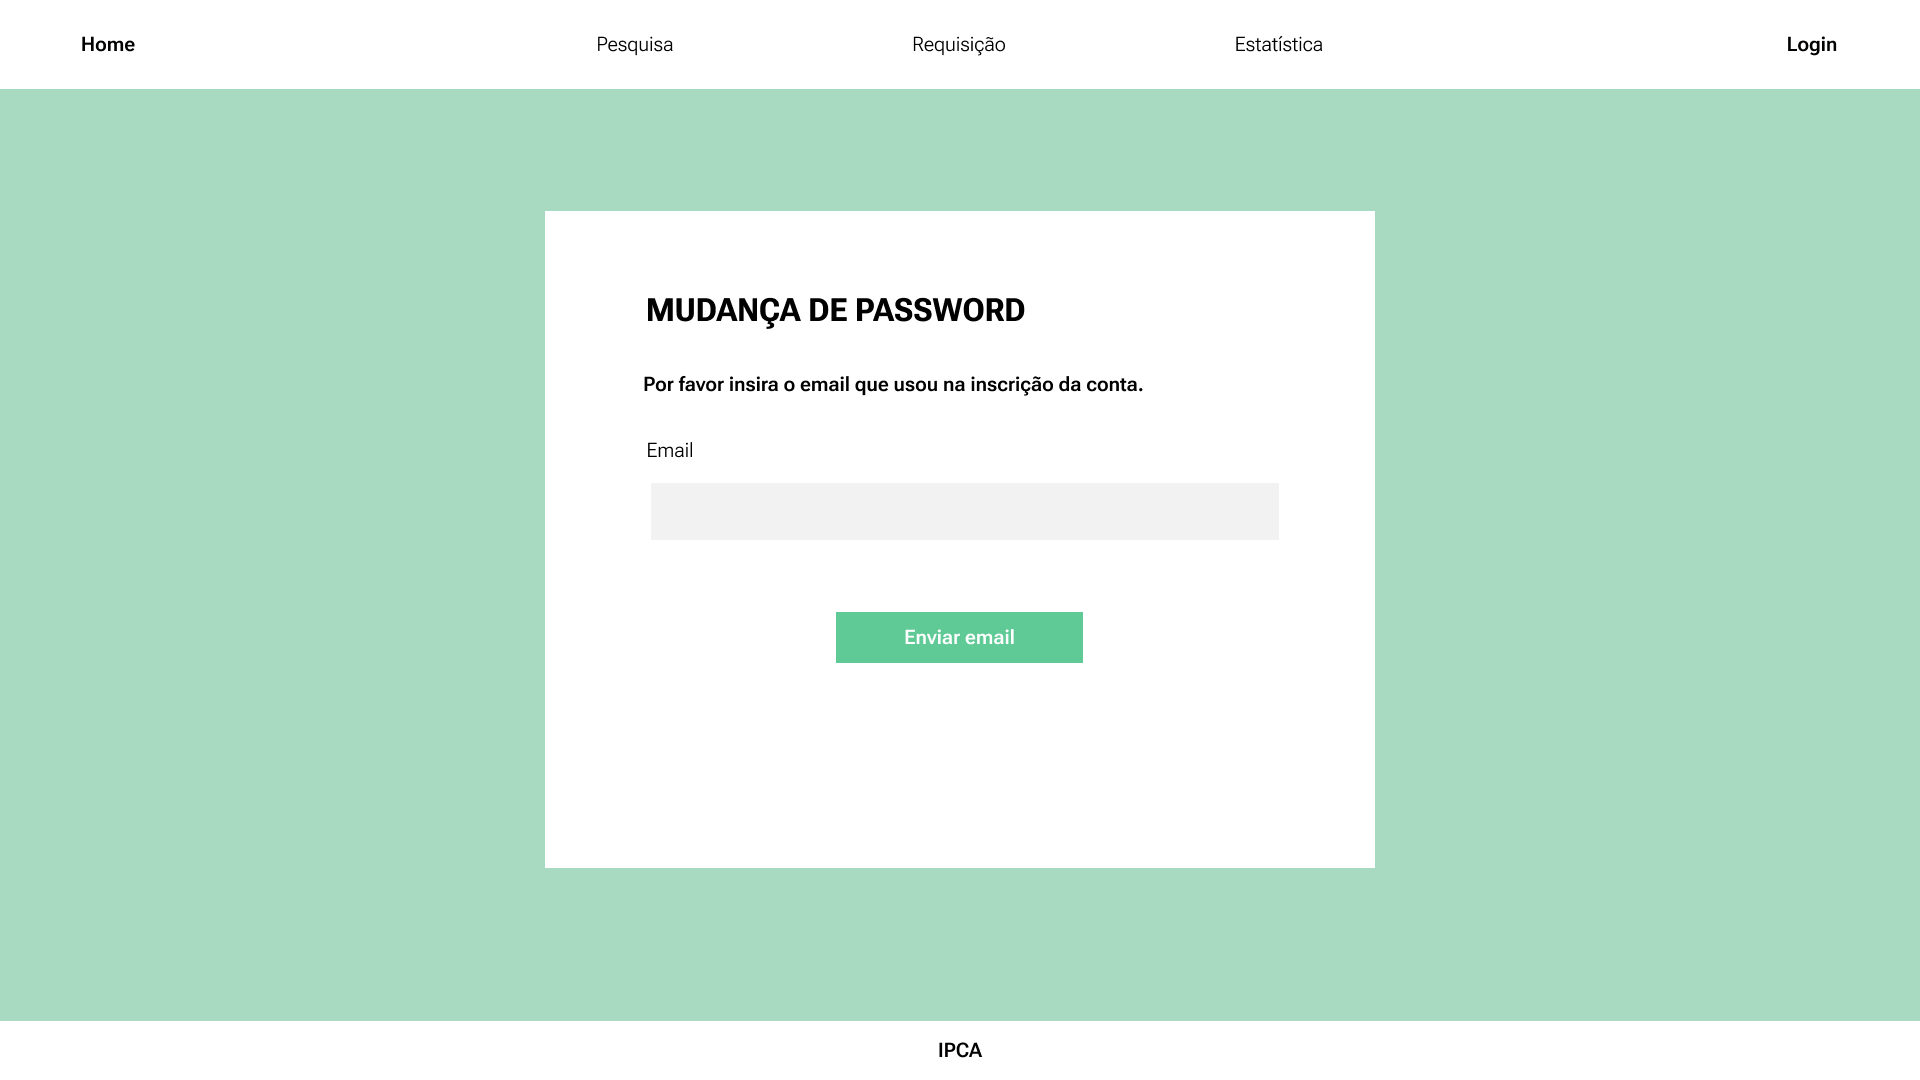
\includegraphics[width=1\linewidth]{../Mockups/PNGs/Login - Password.png}  % largura percentual 
	\caption{\ref{mo:272}}
	\label{fig:chap272}
\end{figure}


\newpage

\subsection{\labeltext[Ecrã - Login Confirmação]{Ecrã - Login Confirmação}{mo:273}}

Pop-up na pagina de Login - Password, a confirmar que o email, foi enviado com smoesso acompanhado de um pequeno aviso caso algo se encontre errado no email.

\begin{figure}[H]
	\centering
	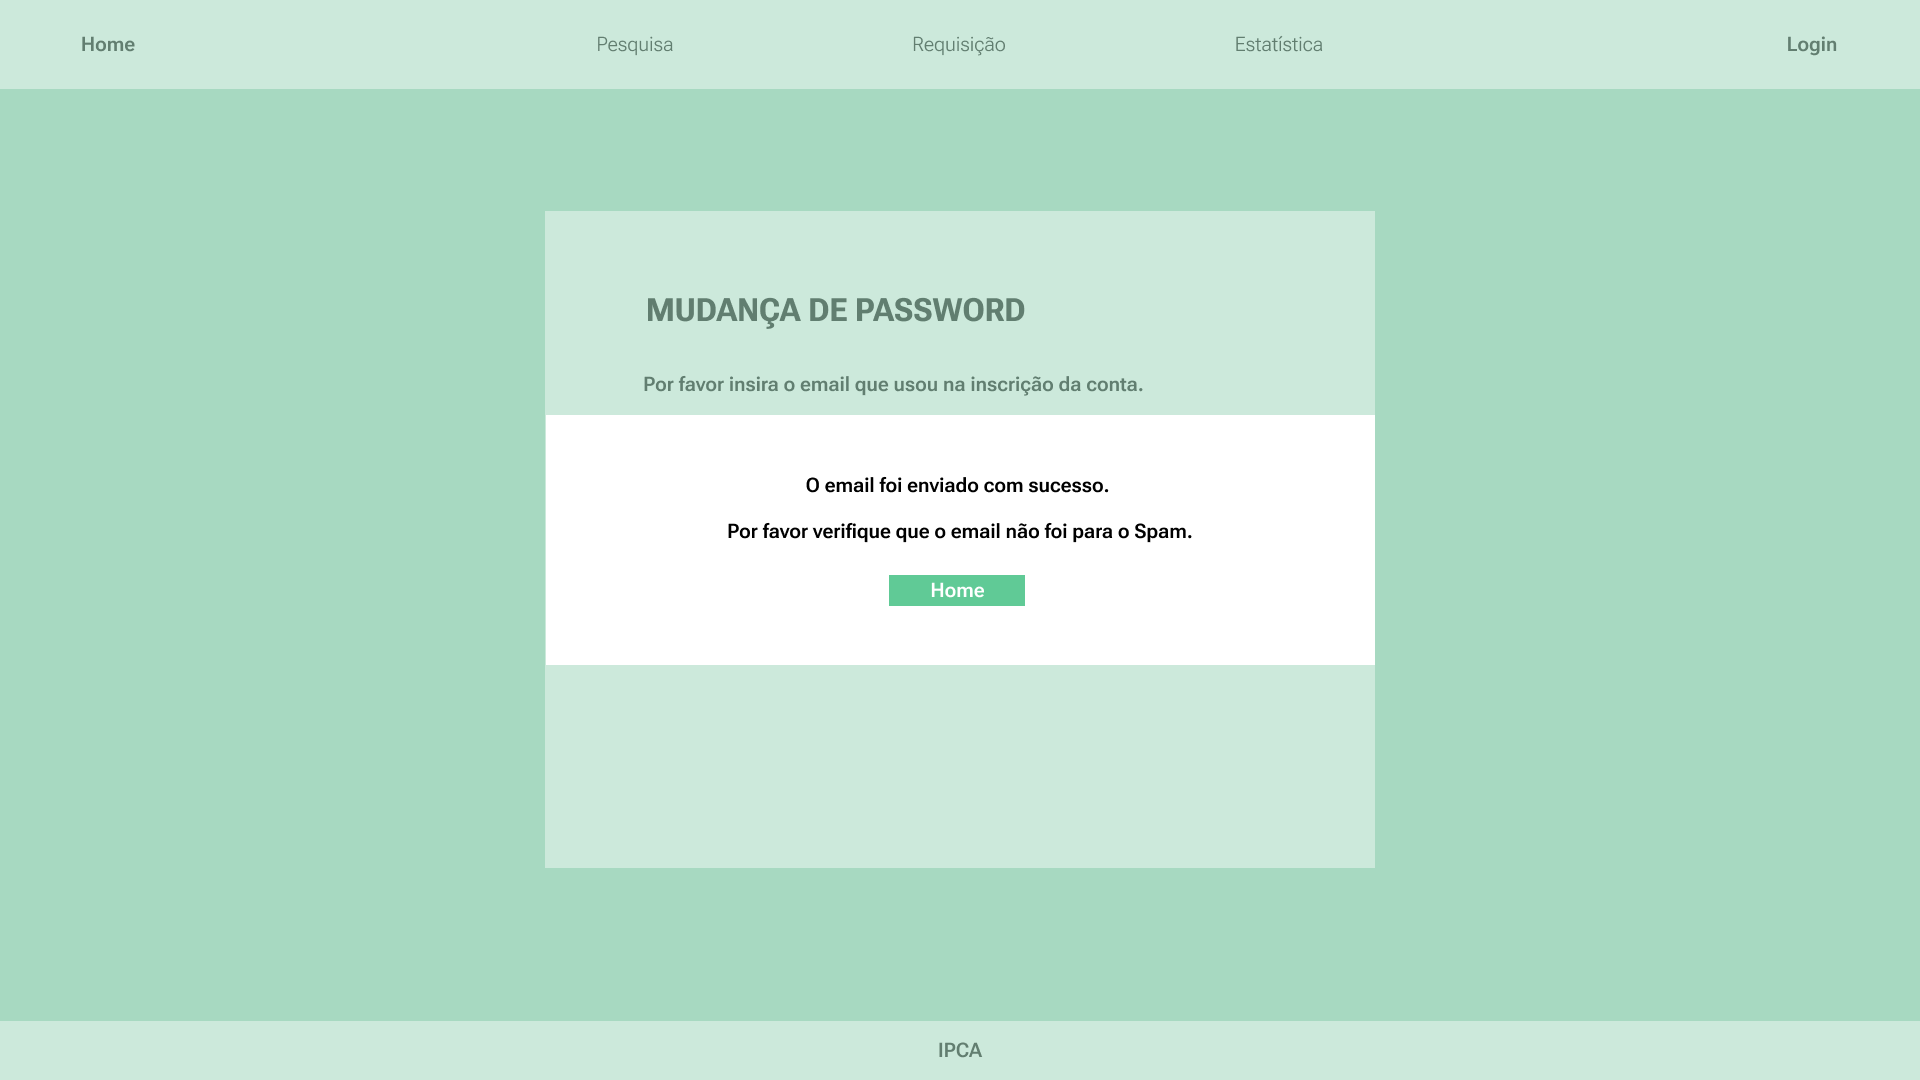
\includegraphics[width=1\linewidth]{../Mockups/PNGs/Login - Password confirmacao.png}  % largura percentual 
	\caption{\ref{mo:273}}
	\label{fig:chap273}
\end{figure}


\newpage 

\subsection{\labeltext[Ecrã - Perfil Utilzador]{Ecrã - Perfil Utilzador}{mo:274}}

A pagina onde o utilizador pode ver a sua informação privada. É possivel também alterar qualquer informação desta pagina caso o mesmo pretenda.

\begin{figure}[H]
	\centering
	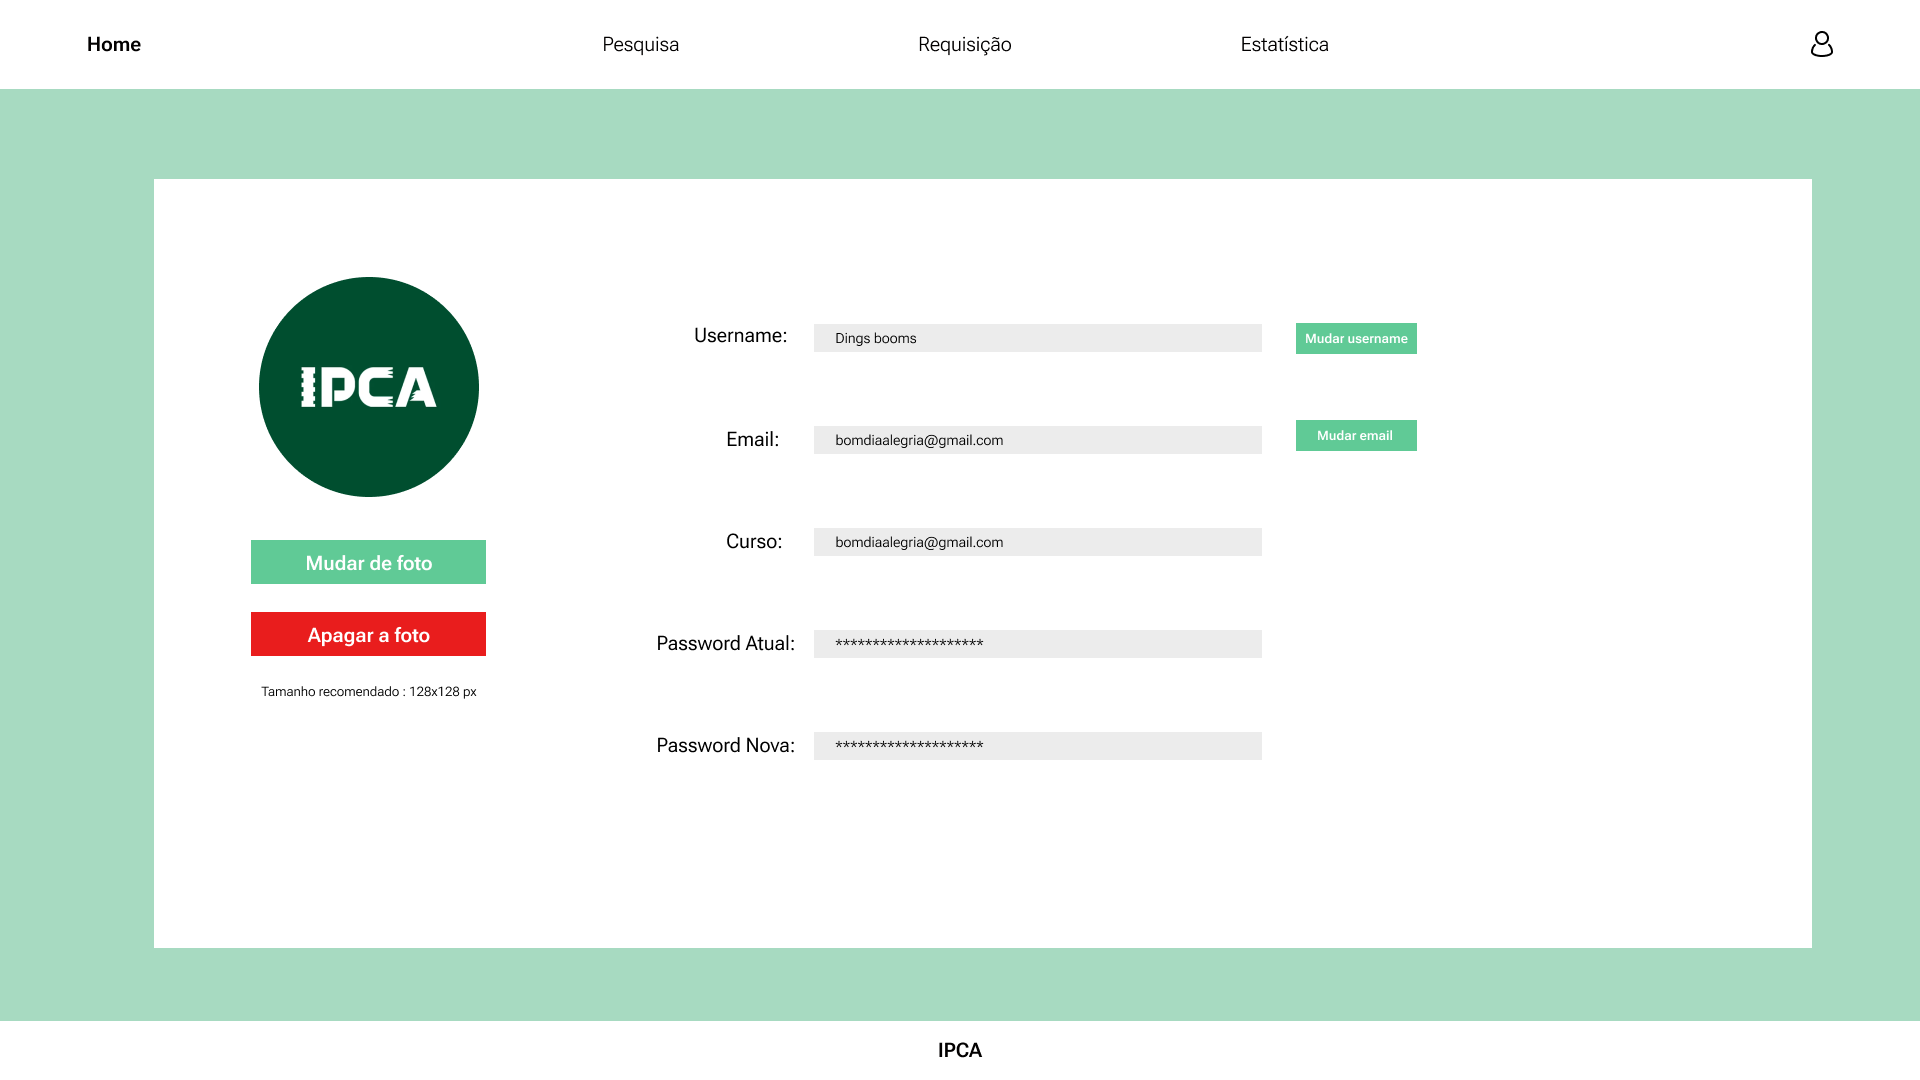
\includegraphics[width=1\linewidth]{../Mockups/PNGs/Perfil do utilizador.png}  % largura percentual 
	\caption{\ref{mo:274}}
	\label{fig:chap274}
\end{figure}

\newpage

\subsection{\labeltext[Ecrã - Pesquisa]{Ecrã - Pesquisa}{mo:275}}

Aqui se encontra a pagina onde é possível fazer a pesquisa dos livros da database e ao mesmo tempo ver se estão disponíveis para serem requisitados. Cada livro vêm com as suas especificações ao lado para o utilizador ver e perceber, se é mesmo o livro que pretendia. 

\begin{figure}[H]
	\centering
	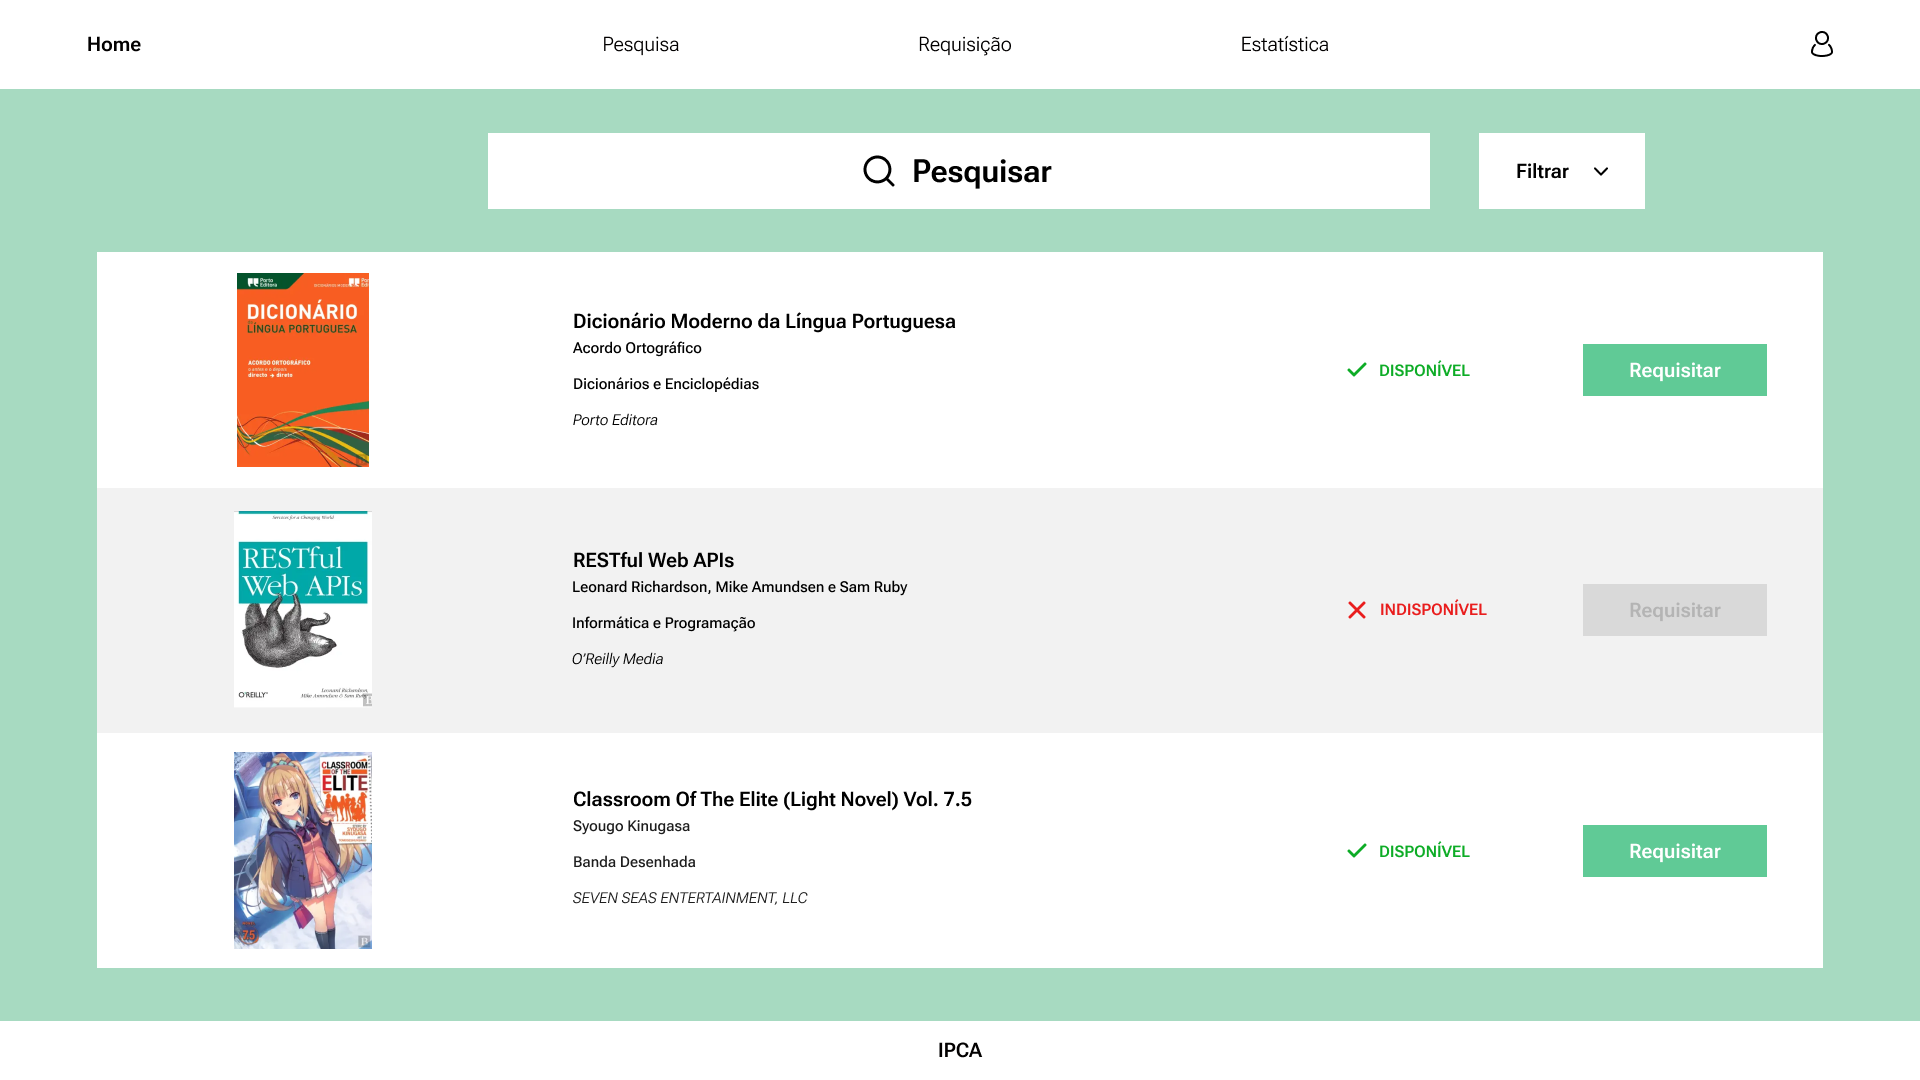
\includegraphics[width=1\linewidth]{../Mockups/PNGs/Pesquisa dos livros.png}  % largura percentual 
	\caption{\ref{mo:275}}
	\label{fig:chap275}
\end{figure}

\newpage 

\subsection{\labeltext[Ecrã - Requisição]{Ecrã - Requisição}{mo:276}}

Pop-up da página anterior onde é escolhido a data de entrega e de limite da requisição como também o numero de exemplares que pretende requisitar.

\begin{figure}[H]
	\centering
	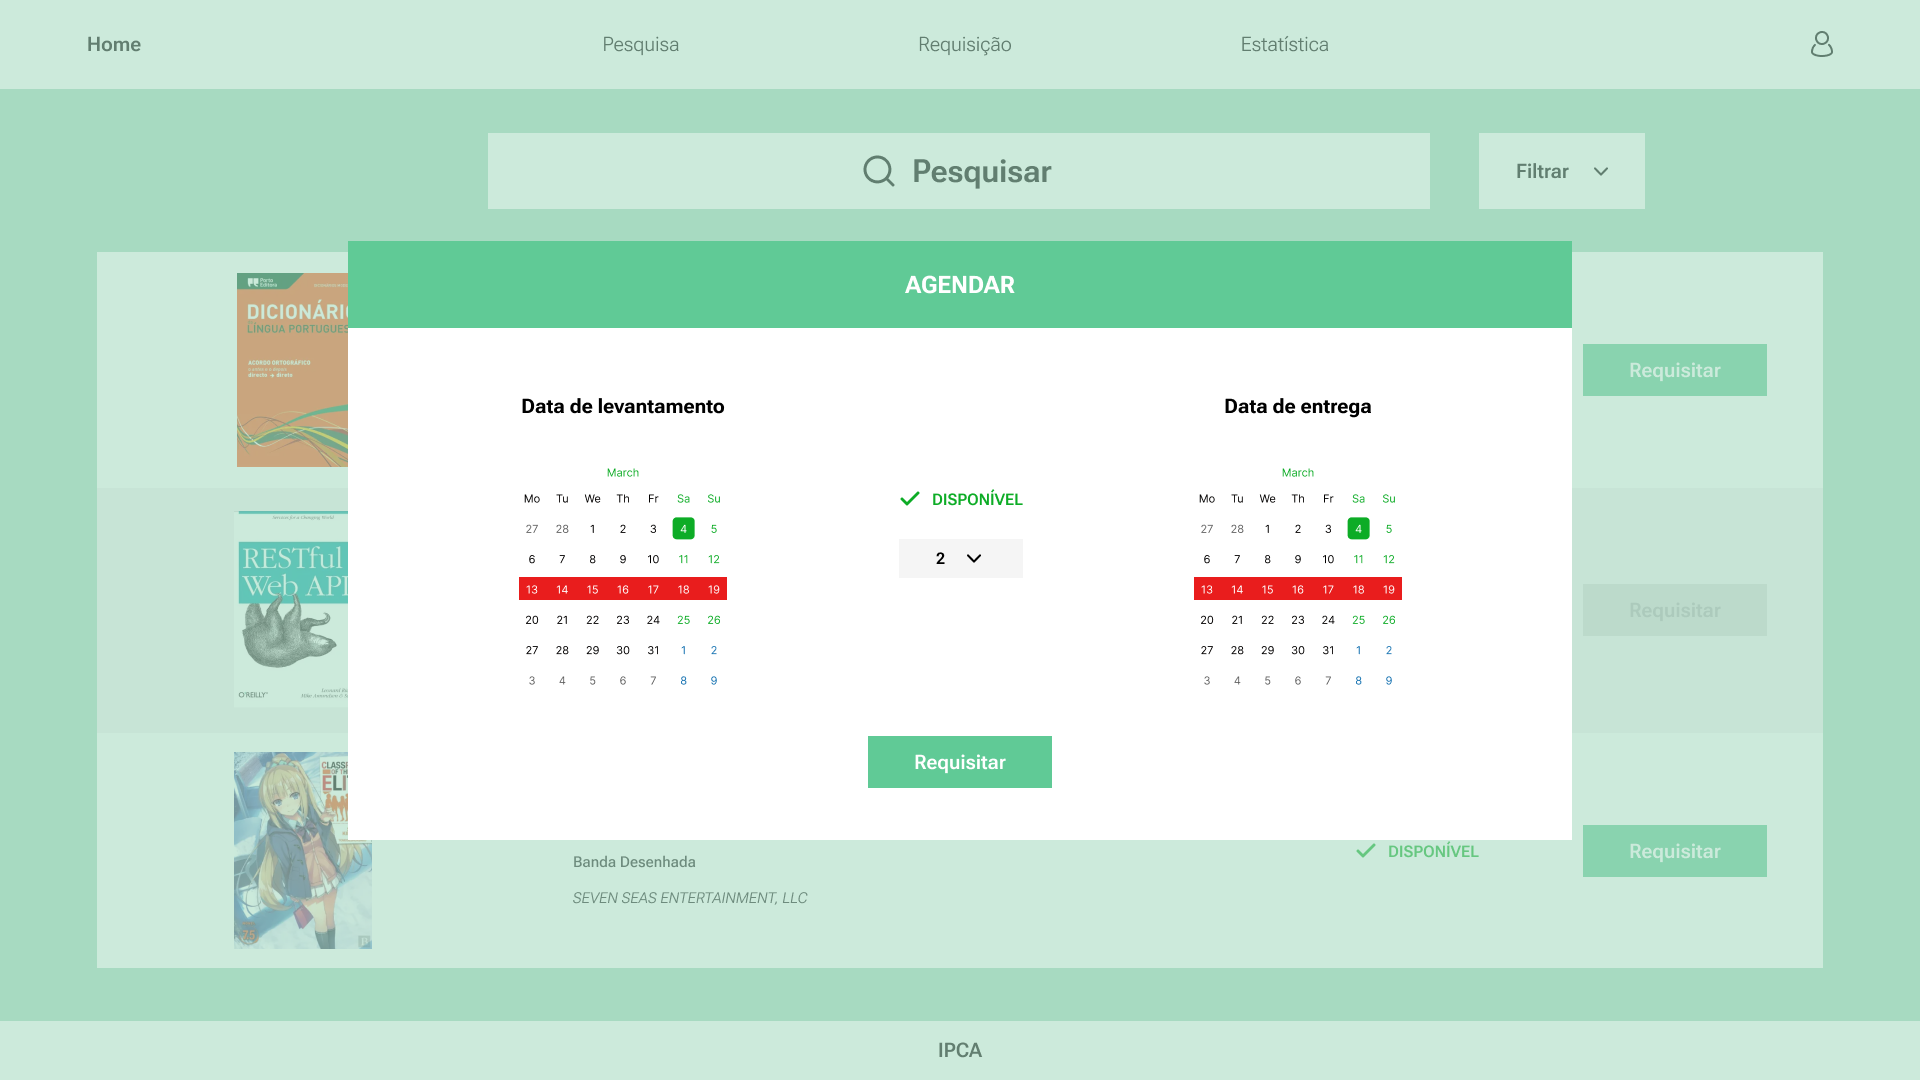
\includegraphics[width=1\linewidth]{../Mockups/PNGs/Agendar Requisitar.png}  % largura percentual 
	\caption{\ref{mo:276}}
	\label{fig:chap276}
\end{figure}


\newpage

\subsection{\labeltext[Ecrã - Minhas Requisições]{Ecrã - Requisições}{mo:277}}

Pagina do utilizador, onde encontram-se as requisições feitas pelo mesmo. Coimas e data de limite da requisição aparecem nesta pagina e as coimas são pagas nesta página ao cliquar no "Expirou".

\begin{figure}[H]
	\centering
	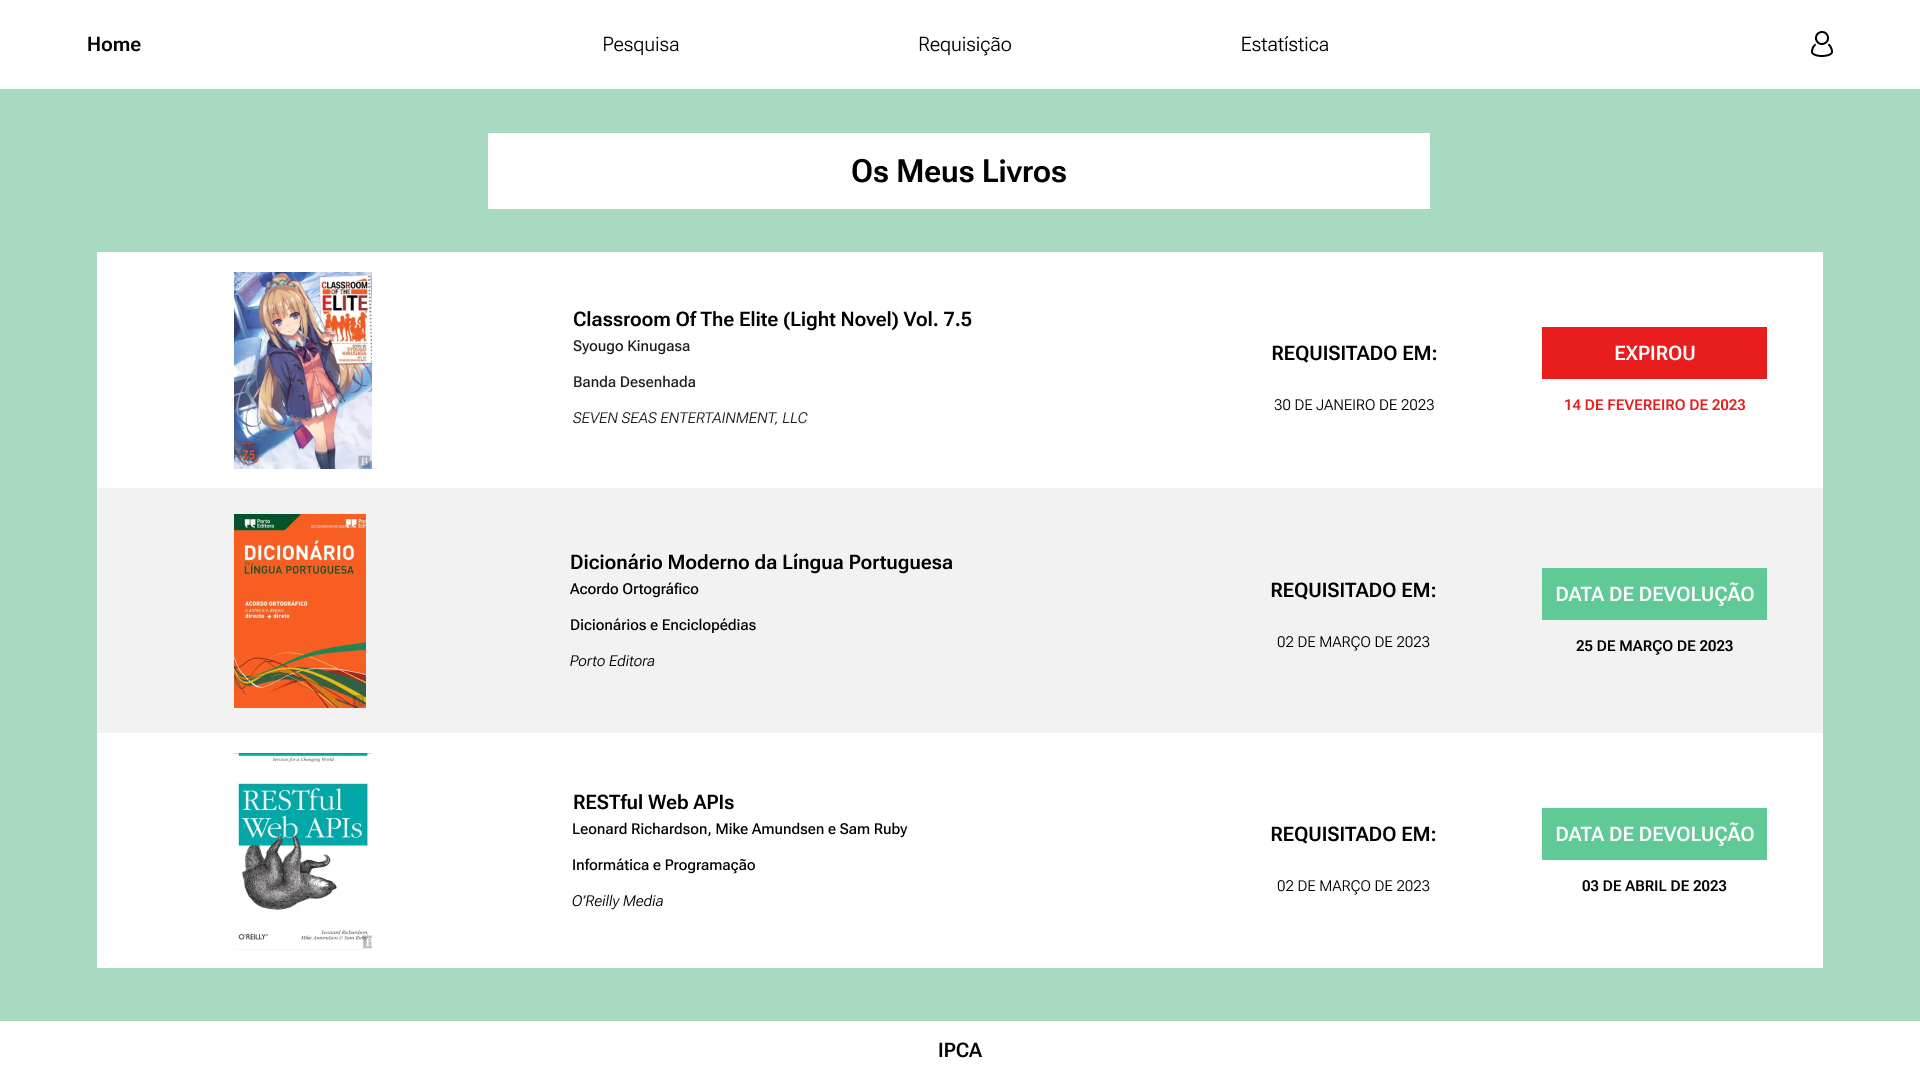
\includegraphics[width=1\linewidth]{../Mockups/PNGs/Minhas Requisicoes.png}  % largura percentual 
	\caption{\ref{mo:277}}
	\label{fig:chap277}
\end{figure}


\newpage

\subsection{\labeltext[Ecrã - Pagamento Multibanco]{Ecrã - Pagamento Multibanco}{mo:278}}

Pop-up da página das "Minhas Requisições" onde vão ser pagas as coimas. Neste ponto é especificado o pagamento por Multibanco.

\begin{figure}[H]
	\centering
	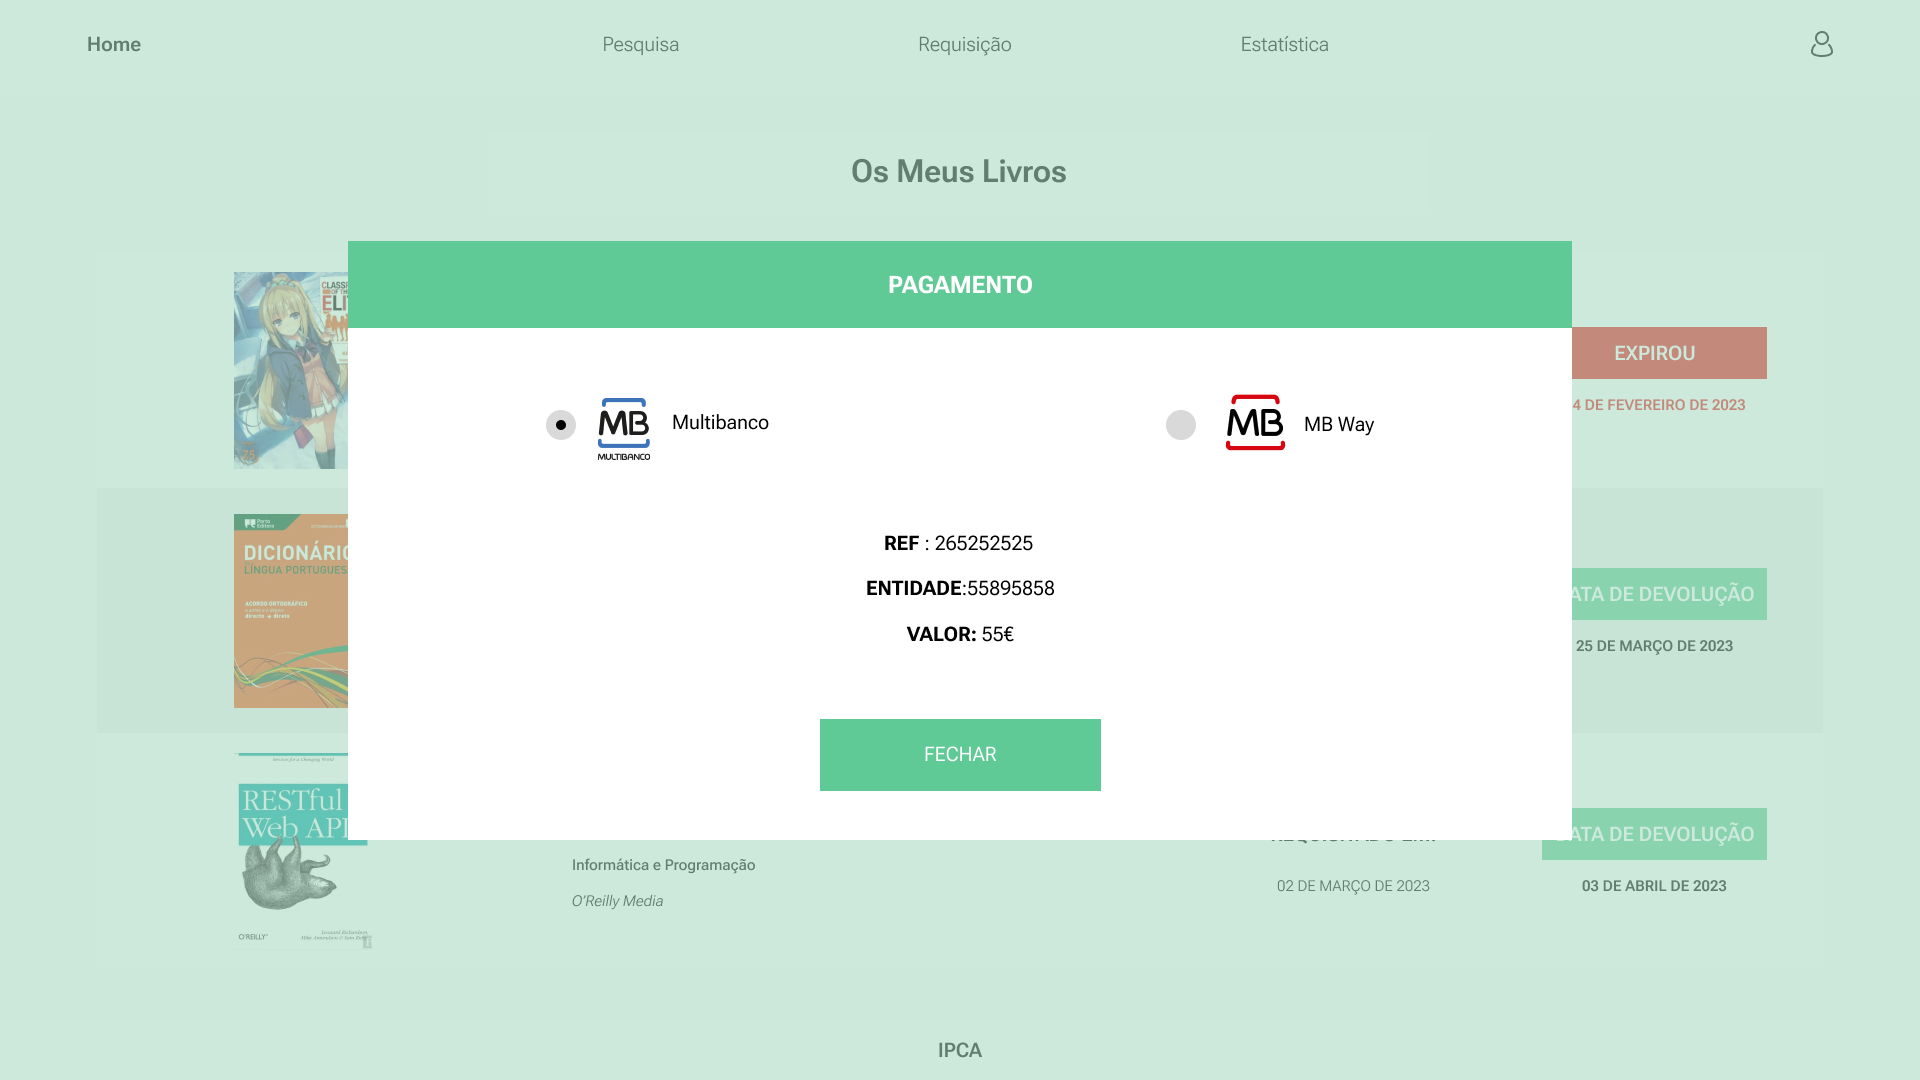
\includegraphics[width=1\linewidth]{../Mockups/PNGs/Pagamento de coimas Multibanco.png}  % largura percentual 
	\caption{\ref{mo:278}}
	\label{fig:chap278}
\end{figure}


\newpage

\subsection{\labeltext[Ecrã - Pagamento MBWay]{Ecrã - Pagamento MBWay}{mo:279}}

Pop-up da página das "Minhas Requisições" onde vão ser pagas as coimas. Neste ponto é especificado o pagamento por MBWay.

\begin{figure}[H]
	\centering
	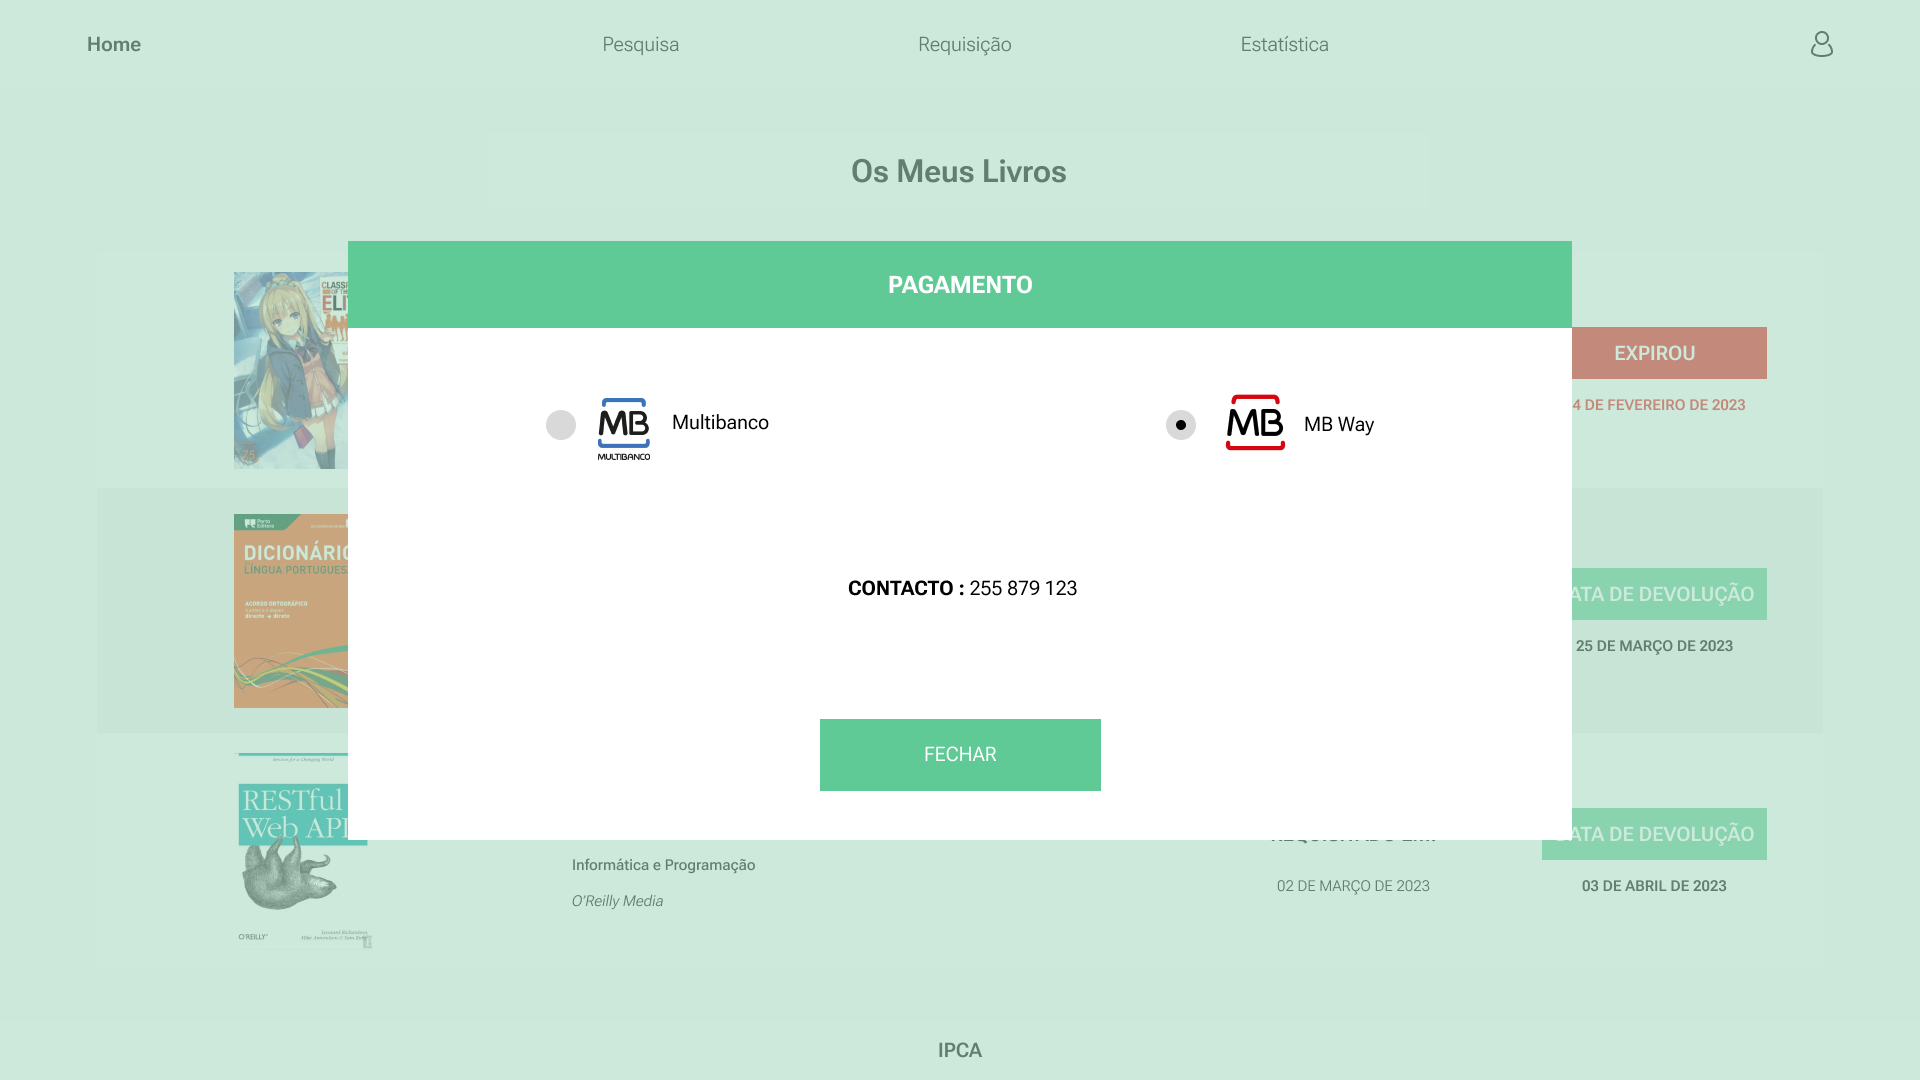
\includegraphics[width=1\linewidth]{../Mockups/PNGs/Pagamento de coimas MBWay.png}  % largura percentual 
	\caption{\ref{mo:279}}
	\label{fig:chap279}
\end{figure}


\newpage

\subsection{\labeltext[Ecrã - Análise de dados 1]{Ecrã - Análise de dados 1}{mo:280}}

Pagina web onde entra a análise e estudo sobre a biblioteca, neste caso em específico uma representação de um gráfico de barras, com uma pequena lista ao seu lado.

\begin{figure}[H]
	\centering
	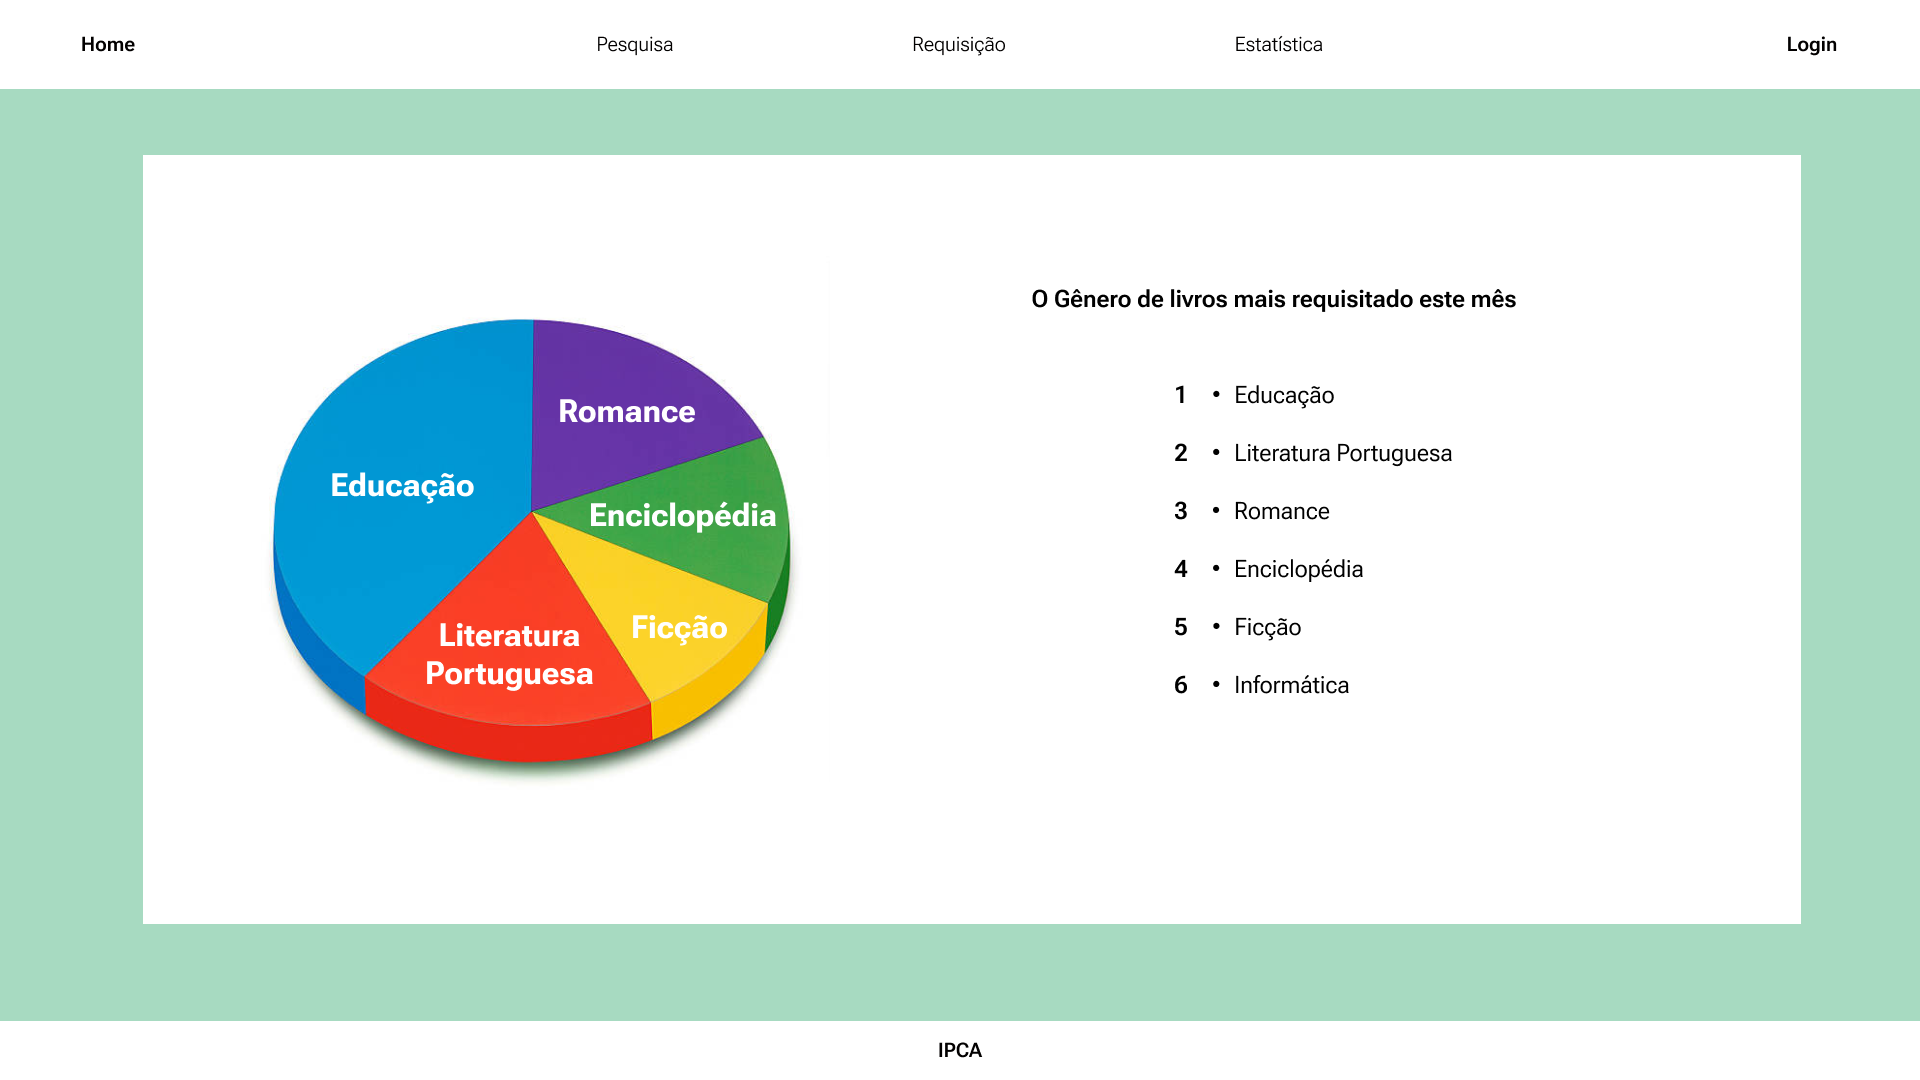
\includegraphics[width=1\linewidth]{../Mockups/PNGs/Estatistica circulo.png}  % largura percentual 
	\caption{\ref{mo:280}}
	\label{fig:chap280}
\end{figure}



\newpage

\subsection{\labeltext[Ecrã - Análise de dados 2]{Ecrã - Análise de dados 2}{mo:281}}

Pagina web onde entra a análise e estudo sobre a biblioteca, neste caso em específico uma representação de um gráfico de barras sobre o estudo do passado ano na biblioteca.

\begin{figure}[H]
	\centering
	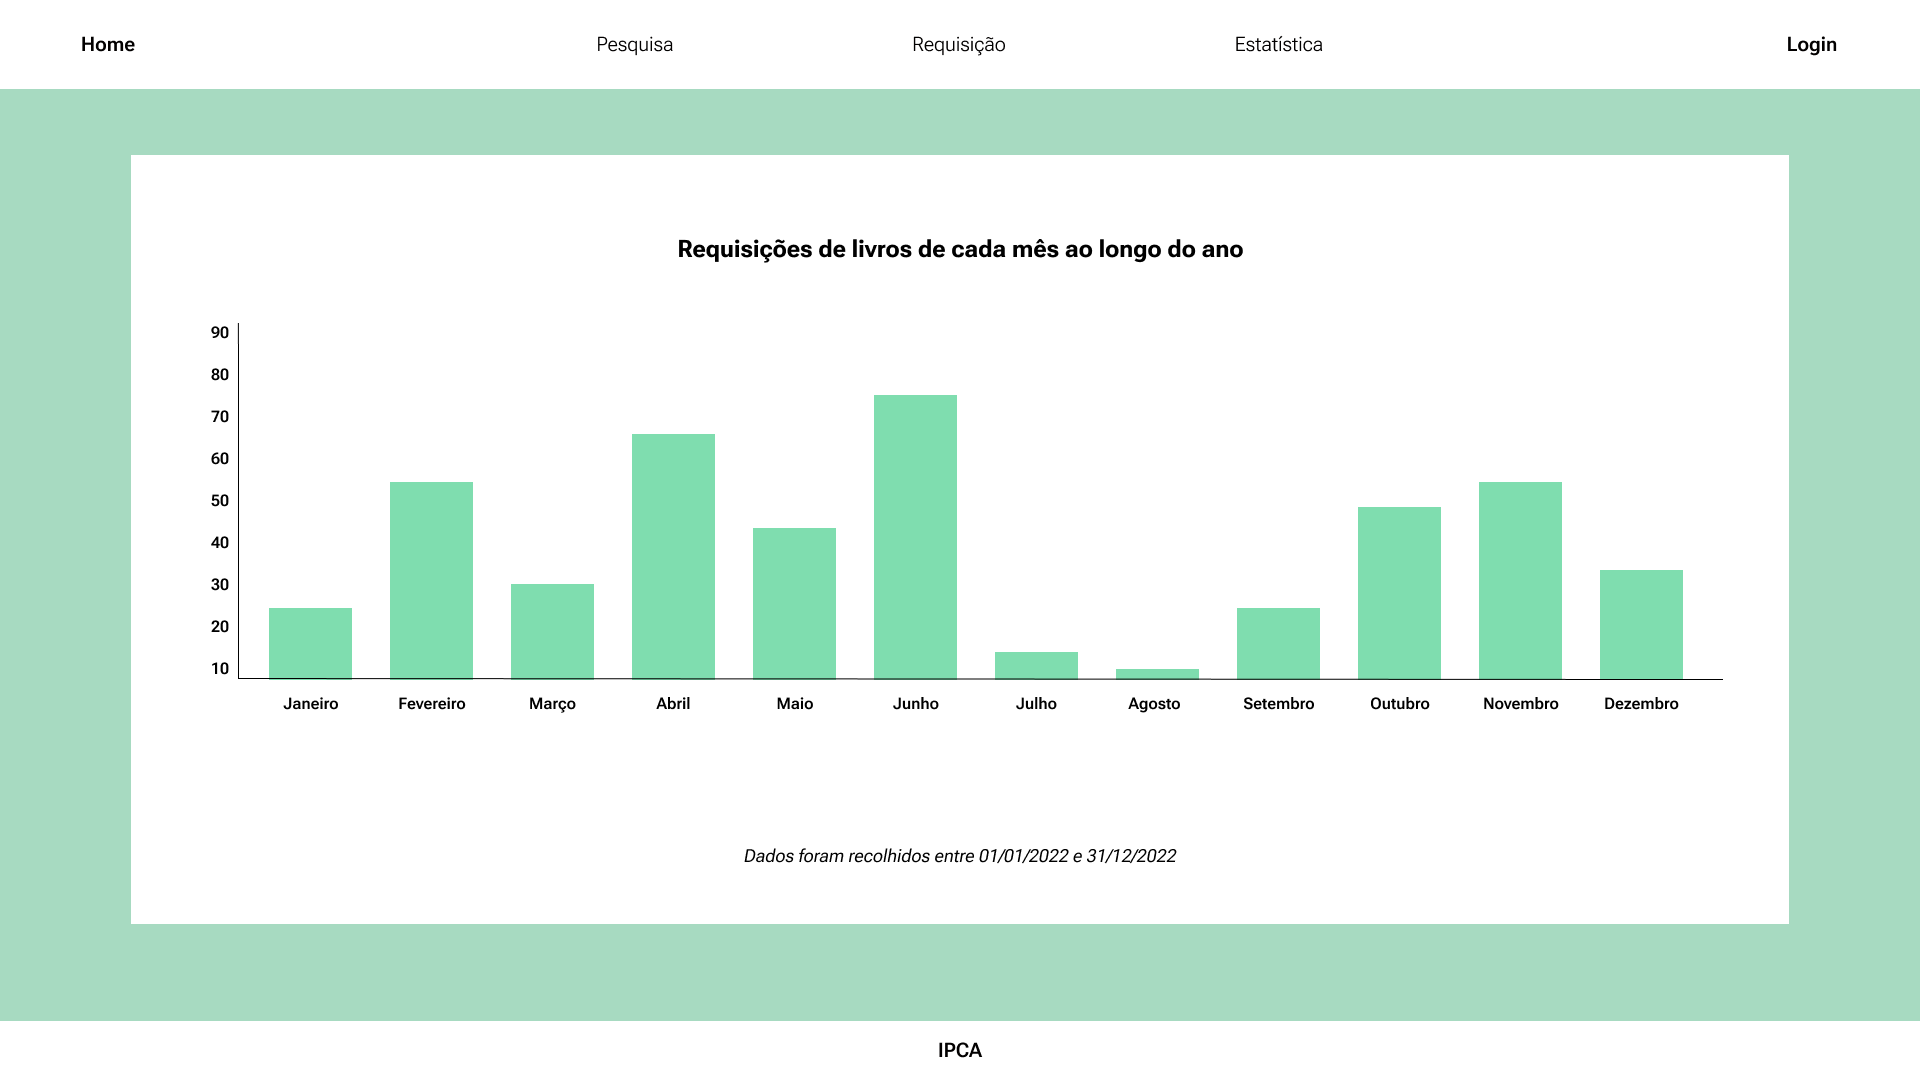
\includegraphics[width=1\linewidth]{../Mockups/PNGs/Estatistica barras.png}  % largura percentual 
	\caption{\ref{mo:281}}
	\label{fig:chap281}
\end{figure}

\newpage

%Reuniões

\section{Milestone Especificação: Reuniões}

\subsection{Reunião ES01}\label{reuniaoES01}

\subsection*{Data: 17/02/2023}


\subsection*{Intervenientes:}
Grupo de trabalho

\subsection*{Temas abordados:}
\begin{itemize}
\item[--] Criação da equipa;
\item[--] Definição do projeto - Ideias de projeto;
\item[--] Definição do projeto - Objetivos;
\item[--] Definição do projeto - Metodologias de trabalho;
\end{itemize}

\noindent Reunir os membros do grupo e atribuir os cargos.

\noindent Após a sugestão de ideas, ficou decidido o sistema base que consiste em desenvolver um sistema web para a biblioteca do IPCA onde as regras de negócio principais são:

\begin{itemize}
\item[--] Requisição de livros;
\item[--] Baixa de livros;
\item[--] Aplicação de coimas;
\item[--] Estatística;
\end{itemize}

\noindent \rule{\linewidth}{0.4pt}
\newline


\newpage

\subsection{Reunião ES02}\label{reuniaoES02}

\subsection*{Data: 24/02/2023}


\subsection*{Intervenientes:}
Grupo de trabalho

\subsection*{Temas abordados:}
\begin{itemize}
\item[--] Desenvolvimento do baclog;
\item[--] Diagramas necessários a serem desenvolvidos;
\item[--] Estruturação do relatório;
\item[--] Destribuição de tarefas;
\end{itemize}

\subsection*{Diagramas a serem desenvolvidos:}

\begin{itemize}
    \item[--] Diagramas de caso de uso;
    \item[--] Diagrama modelo ER;
    \item[--] Diagrama de classes;
    \item[--] Diagrama de estados;
    \item[--] Diagrama de atividades;
    \item[--] Diagrama de sequência;
    \end{itemize}

\noindent \rule{\linewidth}{0.4pt}
\newline


\newpage

\subsection{Reunião ES03}\label{reuniaoES03}

\subsection*{Data: 03/03/2023}


\subsection*{Intervenientes:}
Grupo de trabalho

\subsection*{Temas abordados:}
\begin{itemize}
\item[--] Revisão do trabalho desenvolvido até ao momento;
\end{itemize}

\noindent \rule{\linewidth}{0.4pt}
\newline


\subsection{Reunião ES04}\label{reuniaoES04}

\subsection*{Data: 10/03/2023}


\subsection*{Intervenientes:}
Grupo de trabalho

\subsection*{Temas abordados:}
\begin{itemize}
\item[--] Revisão do trabalho desenvolvido até ao momento;
\item[--] Revisão do relatório; 
\end{itemize}

\noindent \rule{\linewidth}{0.4pt}
\newline


\newpage

\newpage

% Release Alpha

\chapter{Release Alpha}

%planeamento & sprints
\input{chap301}

%reuniões

%reuniões

\subsection{Reunião MA01}\label{reuniaoMA01}

\subsection*{Data:}


\subsection*{Intervenientes:}
Grupo de trabalho

\subsection*{Âmbito:}
\begin{itemize}
\item[--] Iniciar levantamento de requisitos para a elaboração do projeto;
\item[--] Inicialização da documentação.
\end{itemize}

\subsection*{Descrição:}

\noindent Reunir os membros do grupo e atribuir os cargos.

\noindent Após a sugestão de ideas, ficou decidido o sistema base que consiste em:

\noindent Algumas \textit{features} identificadas:

\noindent \rule{\linewidth}{0.4pt}
\newline


% Release Beta

\chapter{Release Beta}

%planeamento & sprints
\input{chap401}

%reuniões
\input{chap450}

% Release ready to web

\chapter{Release to Web}

%planeamento & sprints
\input{chap501}

%reuniões
\input{chap550}


\end{document} 